%%%%%%%%%%%%%%%%%%%%%%%%%%%%%%% main.tex %%%%%%%%%%%%%%%%%%%%%%%%%%%%%%%
%                                                                      %
% --------------------- Report Template IST [EN] --------------------- %
%                                                                      %
%       João Marafuz Gaspar                                            %
%       Departamento de Engenharia Eletrotécnica e de Computadores     %
%       Instituto Superior Tecnico                                     %
%       Av. Rovisco Pais                                               %
%       1049-001 Lisboa                                                %
%       Portugal                                                       %
%       E-mail: joao.marafuz.gaspar@tecnico.ulisboa.pt                 %
%                                                                      %
%  Created:       Jul 30, 2022                                         %
%  Last Modified: Apr 6, 2023                                          %
%                                                                      %
%%%%%%%%%%%%%%%%%%%%%%%%%%%%%%%%%%%%%%%%%%%%%%%%%%%%%%%%%%%%%%%%%%%%%%%%
%  Revision history                                                    %
%  v1 - 2022/07/30 - original template                                 %
%  v2 - 2023/04/06 - change superscript in the cover, updated font,    %
%                    added subfigures and table                        %
%%%%%%%%%%%%%%%%%%%%%%%%%%%%%%%%%%%%%%%%%%%%%%%%%%%%%%%%%%%%%%%%%%%%%%%%
%                              Preamble                                %
%%%%%%%%%%%%%%%%%%%%%%%%%%%%%%%%%%%%%%%%%%%%%%%%%%%%%%%%%%%%%%%%%%%%%%%%

% ----------------------------------------------------------------------
% Set the document class
% ----------------------------------------------------------------------
\documentclass[11pt]{article} % SET FONT SIZE
\usepackage{times} % TIMES NEW ROMAN
% ----------------------------------------------------------------------
% Define external packages, language, margins, fonts, new commands 
% and colors
% ----------------------------------------------------------------------
\usepackage[utf8]{inputenc} % Codification
\usepackage[english]{babel} % Writing idiom

\usepackage[export]{adjustbox} % Align images
\usepackage{amsmath} % Extra commands for math mode
\usepackage{amssymb} % Mathematical symbols
\usepackage{anysize} % Personalize margins
    \marginsize{2cm}{2cm}{2cm}{2cm} % {left}{right}{above}{below}
\usepackage{appendix} % Appendices
\usepackage{cancel} % Expression cancellation
\usepackage{caption} % Captions
    \DeclareCaptionFont{newfont}{\fontfamily{cmss}\selectfont}
    \captionsetup{labelfont={bf, newfont}}
\usepackage{cite} % Citations, like [1 - 3]
\usepackage{color} % Text coloring
\usepackage{fancyhdr} % Head note and footnote
    \pagestyle{fancy}
    \fancyhf{}
    \fancyhead[L]{\footnotesize \fontfamily{cmss}\selectfont Usability Report} % Left of Head note
    \fancyhead[R]{\footnotesize \fontfamily{cmss}\selectfont Hypermedia Applications} % Right of Head note
    \fancyfoot[L]{\footnotesize \fontfamily{cmss}\selectfont} % Left of Footnote
    \fancyfoot[C]{\thepage} % Center of Footnote
    \fancyfoot[R]{\footnotesize \fontfamily{cmss}\selectfont} % Right of Footnote
    \renewcommand{\footrulewidth}{0.4pt} % Footnote rule
\usepackage{float} % Utilization of [H] in figures
\usepackage{graphicx} % Figures in LaTeX
\usepackage[colorlinks = false, plainpages = true, linkcolor = istblue, urlcolor = istblue, citecolor = istblue, anchorcolor = istblue]{hyperref}
\usepackage[super]{nth} % Superscripts
\usepackage{siunitx} % SI units
\usepackage{subcaption} % Subfigures
%\usepackage{titlesec} % Font
%    \titleformat{\section}{\fontfamily{cmss}\selectfont\Large\bfseries}{\thesection}{1em}{}
%    \titleformat{\subsection}{\fontfamily{cmss}\selectfont\large\bfseries}{\thesubsection}{1em}{}
%    \titleformat{\subsubsection}{\fontfamily{cmss}\selectfont\normalsize\bfseries}{\thesubsubsection}{1em}{}
%    \fancyfoot[C]{\fontfamily{cmss}\selectfont\thepage}


% Random text (not needed)
\usepackage{lipsum}
\usepackage{duckuments}

% Manually added packages

% New and re-newcommands
\newcommand{\sen}{\operatorname{\sen}} % Sine function definition
\newcommand{\HRule}{\rule{\linewidth}{0.5mm}} % Specific rule definition
\renewcommand{\appendixpagename}{\LARGE \fontfamily{cmss}\selectfont Appendices}

%\titleformat{\paragraph}[hang]{\normalfont\normalsize\bfseries}{\theparagraph}{1em}{}
%\titlespacing*{\paragraph}{0pt}{3.25ex plus 1ex minus .2ex}{0.5em}

% Colors
\definecolor{istblue}{RGB}{3, 171, 230}
\definecolor{dkgreen}{rgb}{0,0.6,0}
\definecolor{gray}{rgb}{0.5,0.5,0.5}

%%%%%%%%%%%%%%%%%%%%%%%%%%%%%%%%%%%%%%%%%%%%%%%%%%%%%%%%%%%%%%%%%%%%%%%%
%                                 Document                             %
%%%%%%%%%%%%%%%%%%%%%%%%%%%%%%%%%%%%%%%%%%%%%%%%%%%%%%%%%%%%%%%%%%%%%%%%
\begin{document}

% ----------------------------------------------------------------------
% Cover
% ----------------------------------------------------------------------
\begin{center}
    \begin{figure}
        \vspace{-1.0cm}
        
\includegraphics[scale = 1, center]{Images/logo_polimi_scritta2.eps} % IST logo
    \end{figure}
    \mbox{}\\[2.0cm]
    \textsc{\Huge Hypermedia Applications}\\[2.5cm]
    \textsc{\LARGE M.Sc. Computer Science \& Engineering}\\[2.0cm]
    \HRule\\[0.4cm]
    {\large \bf {\fontfamily{cmss}\selectfont Usability Report}\\[0.2cm]
    \HRule\\[1.5cm]}
\end{center}

\begin{flushleft}
    \textbf{\fontfamily{cmss}\selectfont Authors:}
\end{flushleft}

\begin{center}
    \begin{minipage}{0.5\textwidth}
        \begin{flushleft}
            Scherini Samuele (10674683)\\
            Sironi Alessandro (10680296)\\
            Tognini Elisa (10699654)\\
        \end{flushleft}
    \end{minipage}%
    \begin{minipage}{0.5\textwidth}
        \begin{flushright}
            \href{mailto:samuele.scherini@mail.polimi.it}{\texttt{samuele.scherini@mail.polimi.it}}\\
            \href{mailto:alessandro1.sironi@mail.polimi.it}{\texttt{alessandro1.sironi@mail.polimi.it}}\\
            \href{mailto:elisa.tognini@mail.polimi.it}{\texttt{elisa.tognini@mail.polimi.it}}
        \end{flushright}
    \end{minipage}
\end{center}
    
\begin{center}
    \large \bf \fontfamily{cmss}\selectfont 2022/2023
\end{center}

\thispagestyle{empty}

\setcounter{page}{0}

\newpage

\paragraph{\huge{Abstract}}
The aim of this Usability Report is to describe the results of the usability assessment carried out on: \href{https://www.theinterngroup.com}{\texttt{The Intern Group website}}. Specifically, the analysis is  performed using the Inspection method and then the User Testing method. The first method involves expert evaluators examining the application interface and evaluating the compliance with recognized usability principles called heuristics. Specifically, the analysis is conducted with reference to the Nielsen and a subset of the MILE heuristics. The User Testing method instead consists of the data collection and observation of how some representatives of real users interact with the system. Its goal is to discover the actual difficulties encountered by the users when interacting  with the website and to obtain systematic feedback on its effectiveness and usability.

\newpage

% ----------------------------------------------------------------------
% Contents
% ----------------------------------------------------------------------
\tableofcontents 

\newpage

% ----------------------------------------------------------------------
% Body
% ----------------------------------------------------------------------
\section{Inspection}
\textit{Usability Inspection} refers to a category of methods used to systematically evaluate the usability of an application, using a team of \textbf{expert evaluators} who have knowledge in the field to carry out the examination. In this section, we will focus on heuristics evaluation, which uses a set of well-known and standardized rules to highlight possible problems. Inspectors will typically thoroughly explore the application, evaluating and judging the compliance with the chosen heuristics. 

\subsection{Inspection Design and General Method}
The methodology and the design applied for the inspection part of the project is described in this section. 
Each evaluator carries an individual, in-depth analysis of the website and the UX-related aspects of the application, by referring to the heuristics defined in the following sections.
The focus is on the look and feel of the elements - such as the overall layout, the interactive elements, the physical properties - and the content displayed in the pages. \\
The usability evaluation is carried out on the entire website, with particular attention in regards to the following elements and pages:
\begin{itemize}
    \item Homepage
    \item Navigation bar (Navbar)
    \item Apply Now Page
    \item Career Fields Page
    \item Destination Page
\end{itemize}

\subsection{Heuristics Definition}
This section defines the heuristics used to conduct the inspection. As studied in the course, the analysis relied on the principles known as \textbf{Nielsen} and \textbf{MILE Heuristics}.
Heuristics can be classified into three main categories:
\paragraph{$\blacksquare$ Presentation heuristics} These heuristics refer to the way the information is presented within the application. They evaluate how the topology of information is implemented, whether information is correctly positioned with respect to consistency, hierarchy and aesthetic.
\paragraph{$\blacksquare$ Navigation heuristics} They evaluate how easily the user can navigate and go from topics to other related ones. 
\paragraph{$\blacksquare$ Content heuristics} At last, these rules evaluate the quality of the actual information content of the site or application. This includes text, images, information quantity, etc. 

\subsubsection{Nielsen Heuristics}
Jakob Nielsen's heuristics (1994) are a set of rules useful for any interactive system, and define the following principles to apply in the development of a website.
Below is a brief but precise explanation of each one, along with the category it belongs to.
\begin{itemize}
    \item \textbf{H1 - Visibility of System Status} \textit{(Presentation)}: This heuristic evaluates whether and how the design of the application keeps the user informed of what is going on, at all times and within a reasonable amount of time. Ways of complying with the heuristics are, for instance, the use of breadcrumbs or orientation maps. 
    \item \textbf{H2 - Match between the System and the Real World} \textit{(Presentation)}: evaluates how the information appears in a natural and logical order, and whether it is conveyed in a language that is familiar to the user.
    \item \textbf{H3 - User Control and Freedom} \textit{(Navigation)}: Users often choose system functions by mistake and will need a clearly marked "emergency exit" to leave the unwanted state without having to go through an extended dialogue. The user must be able to always be in control of what they are doing, rather than being forced through a lengthy procedure to make changes.
    \item \textbf{H4 - Consistency and Standards} \textit{(Presentation)}: Users should not have to wonder whether different words, situations, or actions mean the same thing. The site should use well-known conventions and should be consistent with them in all its pages and contents.
    \item \textbf{H5 - Error Prevention} \textit{(Presentation)}: Evaluates how the site avoids error prone situations and ensures that, before critical paths or decisions are taken, confirmation options are present. 
    Other than making error correction easy, errors should be avoided as much as possible. 
    \item \textbf{H6 - Recognition rather than Recall} \textit{(Presentation)}: this heuristic evaluates how the site provides visible options and instructions at all times so that the user does not have to remember information from one part of the dialogue to another. Recognition must be properly implemented so that the user always has information and context accessible, so that they are not lost.
    \item \textbf{H7 - Flexibility and Efficiency of use} \textit{(Navigation)}: evaluates how the system provides ways of use for all types of users - both novice and experts - and how the user can tailor their experience and frequent actions on the site.
    \item \textbf{H8 - Aesthetic and Minimalist Design} \textit{(Content)}: evaluates how the site only provides the needed information to the user during dialogues: the presence of unnecessary or rarely needed information can be confusing and can diminish the perceived importance of actually relevant aspects. 
    \item \textbf{H9 - Help users recognize, diagnose and recover from errors} \textit{(Presentation)}: error messages should be expressed in plain language (avoiding error codes), precisely indicate the problem and constructively suggest a solution.
    \item \textbf{H10 - Help and Documentation} \textit{(Content)}: even though it is better if the system can be used without documentation, it may be necessary to provide help and documentation. Any such information should be easy to search, focused on the user's task, list concrete steps to be carried out, and not be too large.
\end{itemize}

\subsubsection{MILE Heuristics}
These heuristics are a larger set of heuristics which focuses on different aspects in a more specific manner. For our purposes, we only chose a subset that was of particular relevance for the task at hand.
\begin{itemize}
    \item \textbf{M1 - Interaction Consistency} \textit{(Navigation)}: evaluates whether pages of the same type have the same navigation links and the same interaction capabilities across the site.
    \item \textbf{M2-1 - Group Navigation 1} \textit{(Navigation)}: evaluates whether menus create cognitive overload, in order to ensure proper understanding of the options the menu is presenting, without creating frustration for the user.
    \item \textbf{M2-2 - Group Navigation 2} \textit{(Navigation)}: evaluates whether menus create cognitive overload, in order to ensure proper understanding of the options the menu is presenting, again without creating frustration for the user. 
    \item \textbf{M3 - Structural Navigation} \textit{(Navigation)}: evaluates the ease of navigation between various sections or parts of the same topic.
    \item \textbf{M4 - Semantic Navigation} \textit{(Navigation)}: evaluates how easily users are able to navigate between related topics, in all directions from one element to the next or previous one.
    \item \textbf{M5 - Landmarks} \textit{(Navigation)}: evaluates whether the landmarks (sections with roles important enough for the user to want to reach and navigate to them quickly) actually aid in recognizing and reaching the most relevant parts of the website.
    \item \textbf{M6 - Information Overload} \textit{(Content)}: evaluates whether the quantity of information contained in a page is adequate - it shouldn't be too much as it would overwhelm the user, but it shouldn't be too little either as pages need to be useful.
    \item \textbf{M7 - Interaction Placeholders: Semiotics} \textit{(Presentation)}: evaluates whether interaction elements are easy to understand, and if the symbols or icons used to present them actually convey their function.
    \item \textbf{M8 - Interaction Placeholders: Consistency} \textit{(Presentation)}: considers whether interaction elements, namely their icon or textual elements, are consistent across the site.
    \item \textbf{M9-1 - Spatial Allocation 1} \textit{(Presentation)}: evaluates whether the on-screen placement of visual elements reflects their importance and relevance.
    \item \textbf{M10 - Consistency of Page Spatial Structure} \textit{(Presentation)}: evaluates whether pages of the same type have the same spatial organization for the various elements that are presented.
    \item \textbf{M11 - Text Layout} \textit{(Presentation)}: considers how well the text can be read and if, for example, spatial arrangement of text is adequate and font size is appropriate.
    \item \textbf{M12 : Consistency of Visual Elements }\textit{(Presentation)}
	evaluates whether, in pages of the same type, visual elements have the same meaning and functional properties. 
    \item \textbf{M13: Hierarchy 1 } \textit{(Presentation)}
	evaluates whether the on-screen placement of contents reflects their importance and relevance. 
    \item \textbf{M14: Hierarchy 2 } \textit{(Presentation)}
	evaluates whether the on-screen placement of visual elements reflects their importance and relevance.
    \item \textbf{M15 : Consistency of Page Content Structure  }\textit{(Content)}
evaluates whether pages that present topics of the same category have the same type of elements across the site.
    \item \textbf{M16 : Contextualized Information } \textit{(Content)}
	evaluates whether the page contains adequate information to remind the user of where they are in the site, in order to avoid them feeling lost.
    \item \textbf{M17 : Content Organization - Hierarchy } \textit{(Content)}
	evaluates if the hierarchy of the contents and elements of the page is adequate to the relevance they hold; are elements with more importance higher in the topological hierarchy. This can be achieved with spatial disposition of contents, their dimension, or other strategies to convey their relevance or lack thereof.
\end{itemize}

\subsection{Metrics Definition}
For each analyzed heuristic, inspectors assign a score which determines how compliant the site is.
The metrics used for the inspection are defined as follows:\\ \\
\begin{center}
    \begin{tabular}{ |c|c| } 
    \hline
    N/A & This heuristic is not applicable \\ 
    \hline
    1 & The heuristic is NOT satisfied; severe violations have been detected \\ 
    \hline
    2 & The heuristic is partly satisfied but it is poorly implemented and must be significantly improved. \\ 
    \hline
    3 & The heuristic is partly satisfied but it can be improved.\\
    \hline
    4 & The heuristic is almost fully satisfied but there are some imperfections. \\
    \hline
    5 & The heuristic is FULLY satisfied; no violation has been detected. \\
    \hline
    \end{tabular}
\end{center}

\subsection{Execution of the study}
To carry out the evaluation, each inspector spent a minimum of 1.5 hours thoroughly exploring the website, carefully analyzing both main and secondary pages. Individual scores for all heuristics were given, which were then discussed by all participants in the inspection. In the following sections, aggregated data about the results of the examination are shown and commented, along with the final scores for each heuristic, decided after discussion of all involved evaluators. 

\subsection{Inspection Execution}
This section reports the evaluations and scores of the heuristics described above, with the correlated screenshot of the identified problems.
\subsubsection{Presentation Heuristics}
In this section the evaluated heuristics are all regarding the presentation category. Following, a graph summarizing the agreed score of the group, along with the average score of the single points attributed by the evaluators.

\begin{figure}[H]
  \centering
  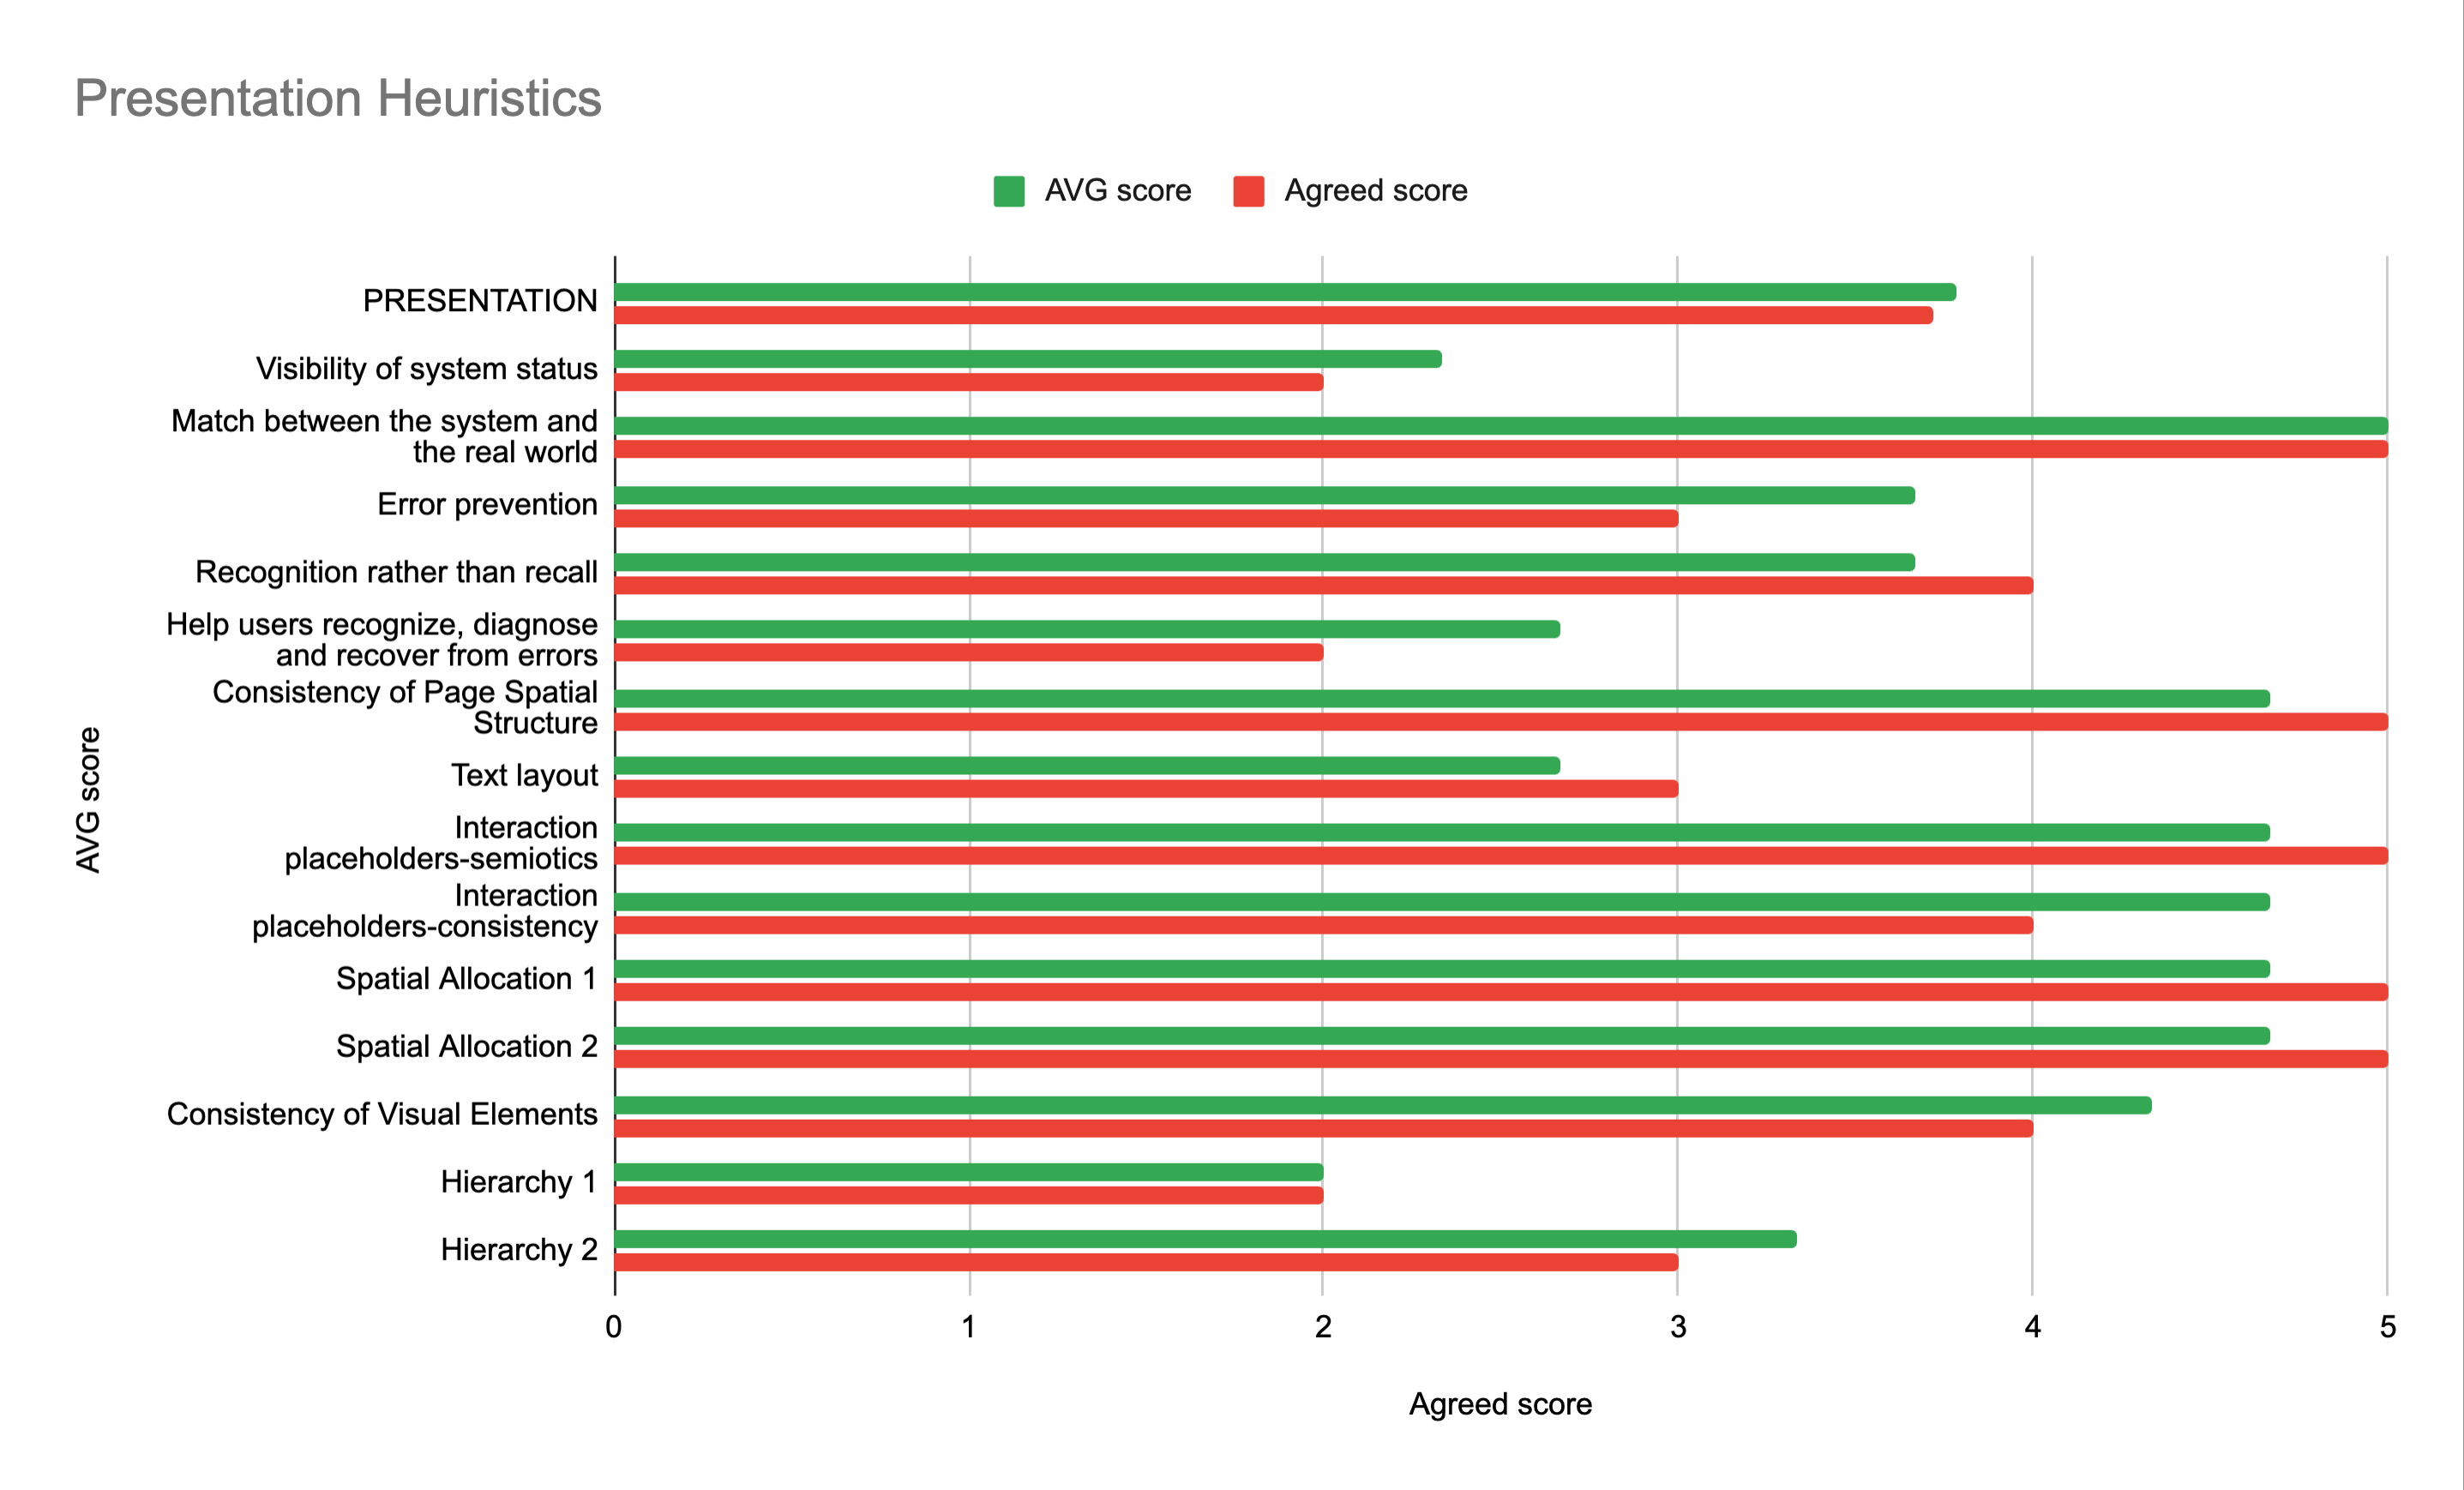
\includegraphics[width=\textwidth]{Images/Presentation Heuristics.png}
  \caption{Presentation Heuristics}
\end{figure}
The average score of all the heuristics regarding the presentation is \textbf{3,7}/5.

%\par\noindent\rule{\textwidth}{0.4pt} 

\paragraph{$\blacksquare$ Visibility of System Status}
\begin{center}
    \begin{tabular}{|c|c|c|}
    \hline
    \textbf{Heuristic Code} & \textbf{Heuristic} & \textbf{Score}\\ 
    \hline
    H1 & Visibility of System Status & 2 \\
    \hline
    \end{tabular}
\end{center}
The problem highlighted by the inspection is that the breadcrumbs, even though present on almost all pages, are too small and hard to see and interact with. The color used often does not offer enough contrast with the background. At last, a few pages do not display them.

\begin{figure}[H]
  \centering
  \includegraphics[width=\textwidth]{Images/Screenshots/Breadcrumbs.png}
  \caption{Breadcrumbs}
\end{figure}

\paragraph{$\blacksquare$ Match between System and Real World}
\begin{center}
    \begin{tabular}{|c|c|c|} 
    \hline
    \textbf{Heuristic Code} & \textbf{Heuristic} & \textbf{Score}\\ 
    \hline
    H2 & Match between System and Real World & 5 \\
    \hline
    \end{tabular}
\end{center}
This heuristic is thought to be fully satisfied by the website. The website uses simple and effective English words and phrases, so that everyone can understand them. Given that the website is offered in English only, all text is uniformly written in the same language.

\paragraph{$\blacksquare$ Error Prevention}
\begin{center}
    \begin{tabular}{|c|c|c|} 
    \hline
    \textbf{Heuristic Code} & \textbf{Heuristic} & \textbf{Score}\\ 
    \hline
    H5 & Error Prevention & 3 \\
    \hline
    \end{tabular}
\end{center}
During the application process (Apply Now), the website correctly alerts whether a required field has been left blank. However, even though following a standard convention, the website uses a "*" red symbol, never explicitly stating what the character stands for. 

\begin{figure}[H]
  \centering
  
\includegraphics[width=0.8\textwidth]{Images/Screenshots/Asterisco Requirements.png}
  \caption{Required Fields}
\end{figure}


\paragraph{$\blacksquare$ Recognition rather than Recall}
\begin{center}
    \begin{tabular}{|c|c|c|} 
    \hline
    \textbf{Heuristic Code} & \textbf{Heuristic} & \textbf{Score}\\ 
    \hline
    H6 & Recognition rather than Recall & 4 \\
    \hline
    \end{tabular}
\end{center}
Apply Now and Contact Us buttons are  visible throughout most of the pages. Also, every choice is aided by a drop-down menu.

\paragraph{$\blacksquare$ Help users recognize, diagnose and recover from errors}
\begin{center}
    \begin{tabular}{|c|c|c|} 
    \hline
    \textbf{Heuristic Code} & \textbf{Heuristic} & \textbf{Score}\\ 
    \hline
    H9 & Help users recognize, diagnose and recover from errors & 2 \\
    \hline
    \end{tabular}
\end{center}
With regards to the "Apply Now" form, the website correctly validates and checks whether the user input is indeed an email or a phone number. However, if some fields are missing or are invalid, you cannot continue filling the form, without any explanation.
The 404 page (Page Not Found error) only allows to go back to the homepage, and does not offer a useful message.

\begin{figure}[H]
  \centering
  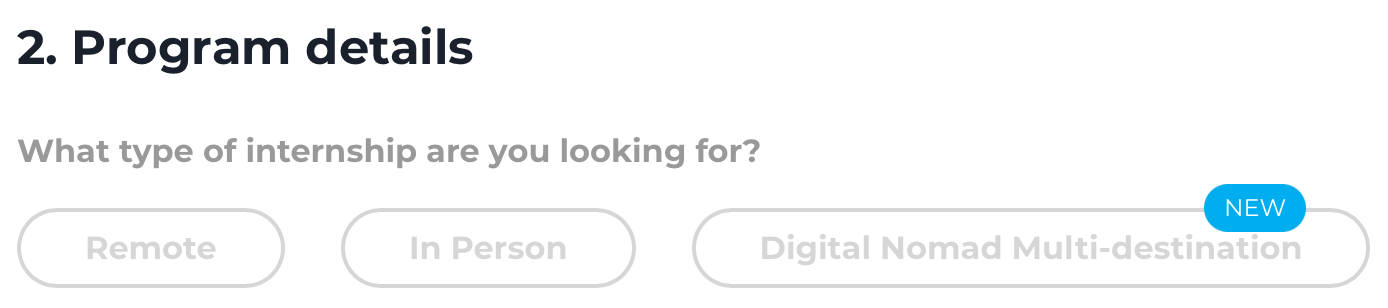
\includegraphics[width=0.5\textwidth]{Images/Screenshots/ApplyNow cant continue.png}
  \caption{No suggestion on why the user can't select any option}
\end{figure}

\begin{figure}[H]
  \centering
  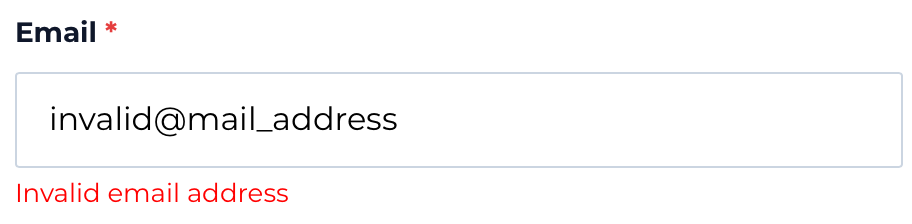
\includegraphics[width=0.5\textwidth]{Images/Screenshots/Invalid Mail Address.png}
  \caption{Error message in form}
\end{figure}

\begin{figure}[H]
  \centering
  
\includegraphics[width=0.7\textwidth]{Images/Screenshots/404.png}
  \caption{404 Page}
\end{figure}

\paragraph{$\blacksquare$ Consistency of Page Spatial Structure}
\begin{center}
    \begin{tabular}{|c|c|c|} 
    \hline
    \textbf{Heuristic Code} & \textbf{Heuristic} & \textbf{Score}\\ 
    \hline
    M10 & Consistency of Page Spatial Structure & 5 \\
    \hline
    \end{tabular}
\end{center}
This heuristic is fully satisfied, as the examined pages of the same category are all structured at the same way.

\paragraph{$\blacksquare$ Text Layout}
\begin{center}
    \begin{tabular}{|c|c|c|} 
    \hline
    \textbf{Heuristic Code} & \textbf{Heuristic} & \textbf{Score}\\ 
    \hline
    M11 & Text Layout & 3 \\
    \hline
    \end{tabular}
\end{center}
The text in the pages is always easy to read and has a well-sized font. However, this is not the case for the breadcrumbs, where the font is too small.

\paragraph{$\blacksquare$ Interaction Placeholders - Semiotics}
\begin{center}
    \begin{tabular}{|c|c|c|} 
    \hline
    \textbf{Heuristic Code} & \textbf{Heuristic} & \textbf{Score}\\ 
    \hline
    M7 & Interaction placeholders - Semiotics & 5 \\
    \hline
    \end{tabular}
\end{center}
The heuristic is fully satisfied. Indeed, the main used icons are the standardized ones and reflect the meaning of the interaction and its effects.

\paragraph{$\blacksquare$ Interaction Placeholders - Consistency}
\begin{center}
    \begin{tabular}{|c|c|c|} 
    \hline
    \textbf{Heuristic Code} & \textbf{Heuristic} & \textbf{Score}\\ 
    \hline
    M7 & Interaction Placeholders - Consistency & 4 \\
    \hline
    \end{tabular}
\end{center}
The different pages all use the same template. However, some arrows often have a different meaning and functionality, risking for the user to exit the page unwillingly.

\paragraph{$\blacksquare$ Spatial Allocation - 1}
\begin{center}
    \begin{tabular}{|c|c|c|} 
    \hline
    \textbf{Heuristic Code} & \textbf{Heuristic} & \textbf{Score}\\ 
    \hline
    M9-1 & Spatial Allocation - 1 & 5 \\
    \hline
    \end{tabular}
\end{center}

\paragraph{$\blacksquare$ Spatial Allocation - 2}
\begin{center}
    \begin{tabular}{|c|c|c|} 
    \hline
    \textbf{Heuristic Code} & \textbf{Heuristic} & \textbf{Score}\\ 
    \hline
    M9-2 & Spatial Allocation - 2 & 5 \\
    \hline
    \end{tabular}
\end{center}
Pages have a simple but efficient layout, consisting of a header for navigation, a body with related articles and a footer with “contact us” information. However there are some pages with a slightly different layout: for example, with a sub-page navigation menu on the left.
The division of the subjects is coherent.

\paragraph{$\blacksquare$ Consistency of Visual Elements}
\begin{center}
    \begin{tabular}{|c|c|c|} 
    \hline
    \textbf{Heuristic Code} & \textbf{Heuristic} & \textbf{Score}\\ 
    \hline
    M12 & Consistency of Visual Elements & 4 \\
    \hline
    \end{tabular}
\end{center}
Throughout the website the same conventions are being put in use, and the buttons are often re-used. However, some buttons with a different functionality are graphically different in the color and shape.

\begin{figure}[H]
  \centering
  
\includegraphics[width=0.3\textwidth]{Images/Screenshots/Chat Button.png}
  \caption{Chat Button}
\end{figure}

\begin{figure}[H]
  \centering
  
\includegraphics[width=0.3\textwidth]{Images/Screenshots/Apply Now Button.png}
  \caption{Apply Now Button}
\end{figure}

\paragraph{$\blacksquare$ Hierarchy - 1}
\begin{center}
    \begin{tabular}{|c|c|c|} 
    \hline
    \textbf{Heuristic Code} & \textbf{Heuristic} & \textbf{Score}\\ 
    \hline
    M13 & Hierarchy - 1 & 2 \\
    \hline
    \end{tabular}
\end{center}

\paragraph{$\blacksquare$ Hierarchy - 2}
\begin{center}
    \begin{tabular}{|c|c|c|} 
    \hline
    \textbf{Heuristic Code} & \textbf{Heuristic} & \textbf{Score}\\ 
    \hline
    M14 & Hierarchy - 2 & 2 \\
    \hline
    \end{tabular}
\end{center}
Navigating the website, every page feels like on the same level of importance. Even though the information written on the pages are inherent with the subject, important facts should stand out from the rest. The content is sometimes unnecessary and repetitive.


\subsubsection{Navigation Heuristics}
\begin{figure}[H]
  \centering
  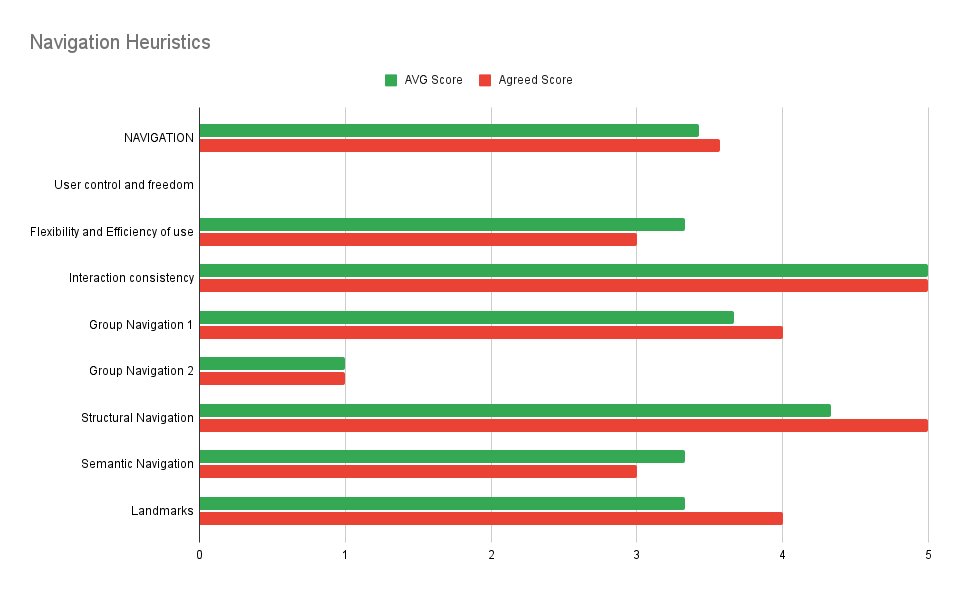
\includegraphics[width=\textwidth]{Images/Navigation Heuristics.png}
  \caption{Navigation Heuristics}
\end{figure}

The average score attributed to all the Navigation Heuristics is \textbf{3,6}/5.

\paragraph{$\blacksquare$ User Control and Freedom}
\begin{center}
    \begin{tabular}{|c|c|c|} 
    \hline
    \textbf{Heuristic Code} & \textbf{Heuristic} & \textbf{Score}\\ 
    \hline
    H3 & User Control and Freedom & N/A \\
    \hline
    \end{tabular}
\end{center}
The heuristic is not considered relevant for the website, as there are not advanced paths that can be taken by the user. 

\paragraph{$\blacksquare$ Flexibility and Efficiency of Use}
\begin{center}
    \begin{tabular}{|c|c|c|} 
    \hline
    \textbf{Heuristic Code} & \textbf{Heuristic} & \textbf{Score}\\ 
    \hline
    H7 & Flexibility and Efficiency of Use & 3 \\
    \hline
    \end{tabular}
\end{center}
The user can reach the same pages, either from the navbar and/or the links at the left edge of the page. However, the navigation through most of navbar links such as the “career fields” are chaotic and inefficient, the career fields are all listed without further categorization or grouping.

\begin{figure}[H]
  \centering
  
\includegraphics[width=\textwidth]{Images/Screenshots/Left Links.png}
  \caption{Links at the edge of the page}
\end{figure}

\paragraph{$\blacksquare$ Interaction Consistency}
\begin{center}
    \begin{tabular}{|c|c|c|} 
    \hline
    \textbf{Heuristic Code} & \textbf{Heuristic} & \textbf{Score}\\ 
    \hline
    M1 & Interaction Consistency & 5 \\
    \hline
    \end{tabular}
\end{center}
The heuristic is satisfied, as similar pages manifest the same behavior.

\paragraph{$\blacksquare$ Group Navigation - 1}
\begin{center}
    \begin{tabular}{|c|c|c|} 
    \hline
    \textbf{Heuristic Code} & \textbf{Heuristic} & \textbf{Score}\\ 
    \hline
    M2-1 & Group Navigation - 1 & 4 \\
    \hline
    \end{tabular}
\end{center}
The heuristic is considered almost fully satisfied, as the navigation is made easy between objects and elements of the same group. 

\paragraph{$\blacksquare$ Group Navigation - 2}
\begin{center}
    \begin{tabular}{|c|c|c|} 
    \hline
    \textbf{Heuristic Code} & \textbf{Heuristic} & \textbf{Score}\\ 
    \hline
    M2-2 & Group Navigation - 2 & 1 \\
    \hline
    \end{tabular}
\end{center}
This heuristic is heavily not satisfied. The navbar is really heavy to navigate, as there are too many options presented to the user, creating a heavy cognitive overload. Breadcrumbs help in the navigation, however not all pages present them. 

\begin{figure}[H]
  \centering
  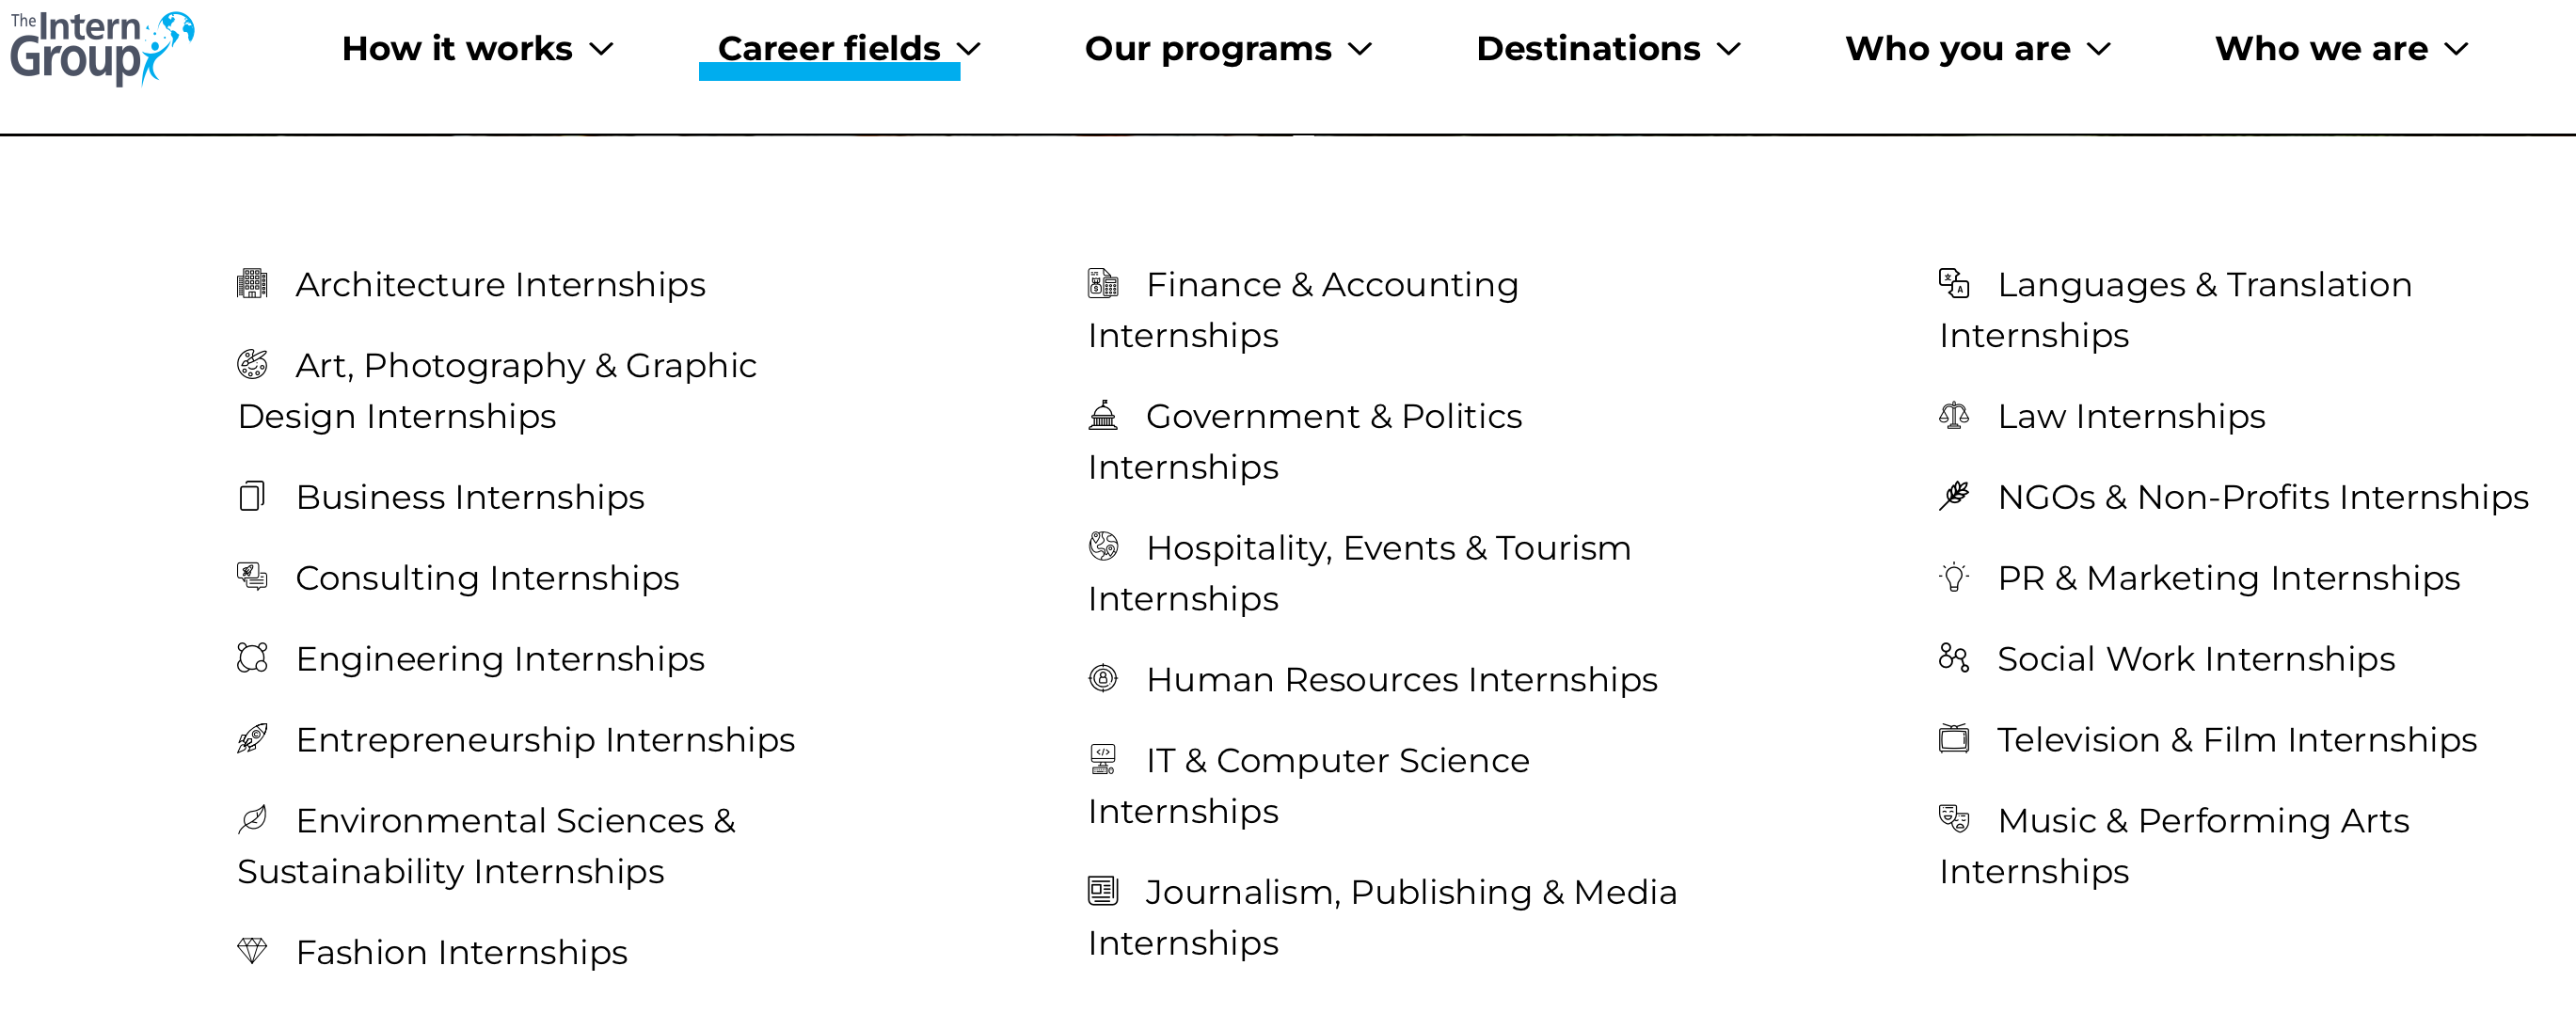
\includegraphics[width=\textwidth]{Images/Screenshots/Career Fields Navbar.png}
  \caption{Career Fields Navbar Menu}
\end{figure}

\paragraph{$\blacksquare$ Structural Navigation}
\begin{center}
    \begin{tabular}{|c|c|c|} 
    \hline
    \textbf{Heuristic Code} & \textbf{Heuristic} & \textbf{Score}\\ 
    \hline
    M3 & Structural Navigation & 5 \\
    \hline
    \end{tabular}
\end{center}
The heuristic is considered satisfied, as many intra-links are present in each page. Also, the side menus helps in the navigation of the pages related to the same subject.

\paragraph{$\blacksquare$ Semantic Navigation}
\begin{center}
    \begin{tabular}{|c|c|c|} 
    \hline
    \textbf{Heuristic Code} & \textbf{Heuristic} & \textbf{Score}\\ 
    \hline
    M4 & Semantic Navigation & 3 \\
    \hline
    \end{tabular}
\end{center}
The navigation between related topics is achieved with the same means covered in the previous heuristic. However, it's not as easy to navigate between career fields or in the blog posts. 

\paragraph{$\blacksquare$ Landmarks}
\begin{center}
    \begin{tabular}{|c|c|c|} 
    \hline
    \textbf{Heuristic Code} & \textbf{Heuristic} & \textbf{Score}\\ 
    \hline
    M5 & Landmarks & 4 \\
    \hline
    \end{tabular}
\end{center}
The heuristic is almost fully satisfied. Home, Apply and Contact Us pages and forms are always reachable, with the exception of a few pages in which the navbar disappears (in particular, in the Employer pages). 


\subsubsection{Content Heuristics}
\begin{figure}[H]
  \centering
  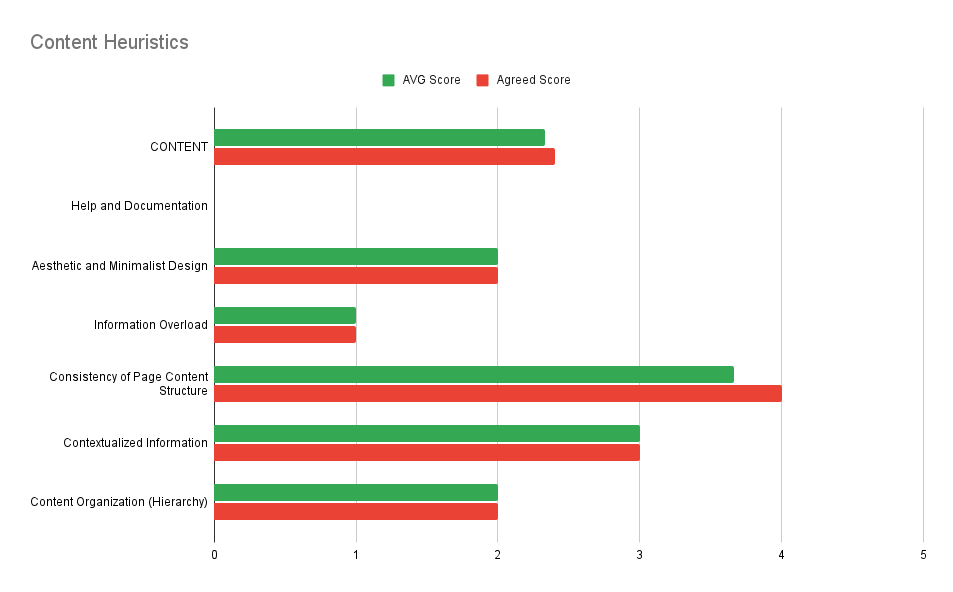
\includegraphics[width=\textwidth]{Images/Content Heuristics.png}
  \caption{Navigation Heuristics}
\end{figure}
The average score attributed to all the Content Heuristics is \textbf{2,4}/5. \\
Comparing to the Presentation and Navigation average heuristics, this is the lowest score.

\paragraph{$\blacksquare$ Help and Documentation}
\begin{center}
    \begin{tabular}{|c|c|c|} 
    \hline
    \textbf{Heuristic Code} & \textbf{Heuristic} & \textbf{Score}\\ 
    \hline
    H10 & Help and Documentation & N/A \\
    \hline
    \end{tabular}
\end{center}
This heuristic is considered not applicable because of a lack of processes that can be documented; the only process a user can take is the "Apply Now", which is deemed straightforward and a single page, therefore not complicated enough to require documentation of any kind.

\paragraph{$\blacksquare$ Aesthetic and Minimalist Design}
\begin{center}
    \begin{tabular}{|c|c|c|} 
    \hline
    \textbf{Heuristic Code} & \textbf{Heuristic} & \textbf{Score}\\ 
    \hline
    H8 & Aesthetic and Minimalist Design & 2 \\
    \hline
    \end{tabular}
\end{center}
The heuristic is considered poorly satisfied. Even though the website is aesthetically pleasing, the pages are too long, with lots of repetitive and useless photos that take a lot of screen space. 
Information could be better split between sub-pages. 

\paragraph{$\blacksquare$ Information Overload}
\begin{center}
    \begin{tabular}{|c|c|c|} 
    \hline
    \textbf{Heuristic Code} & \textbf{Heuristic} & \textbf{Score}\\ 
    \hline
    M6 & Information Overload & 1 \\
    \hline
    \end{tabular}
\end{center}
This heuristic is not satisfied, and is thought to be the biggest problem regarding this website. The pages are dense with information and are too long and make finding information a user might be really interested in too difficult. The homepage contains useless information. 

\begin{figure}[H]
  \centering
  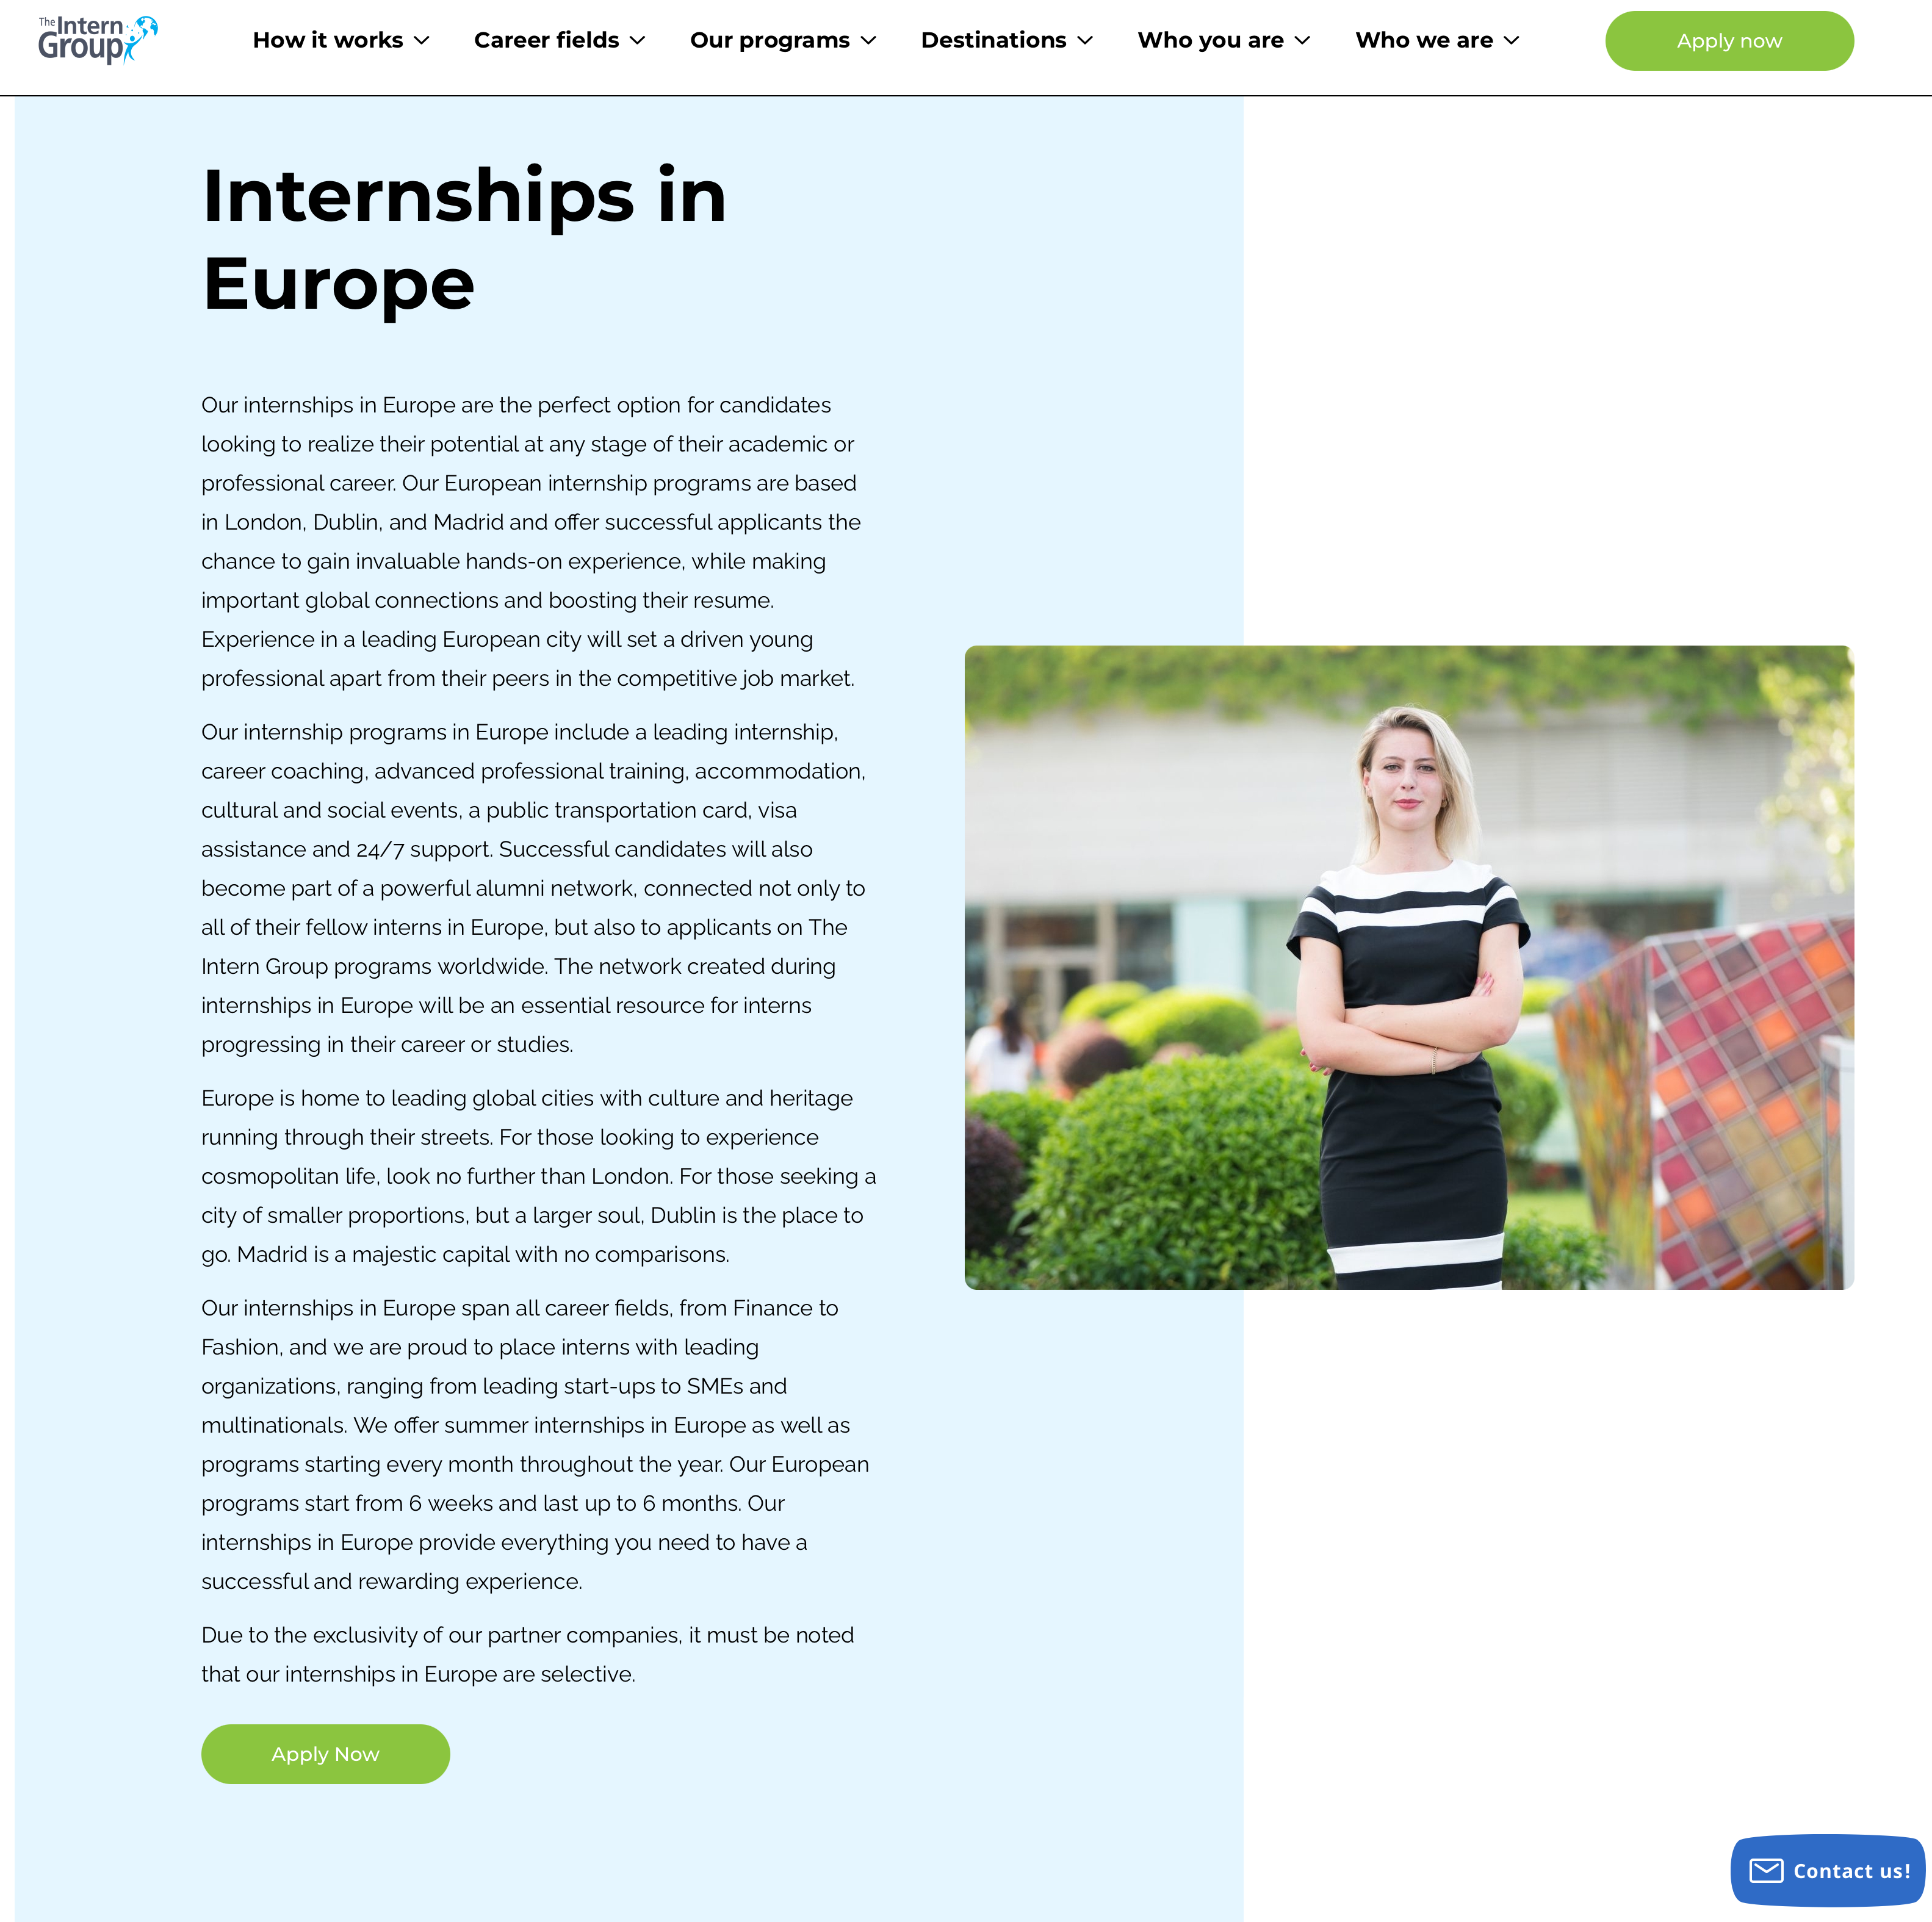
\includegraphics[width=0.8\textwidth]{Images/Screenshots/Wall Of Text.png}
  \caption{Wall of Text}
\end{figure}

\paragraph{$\blacksquare$ Consistency of Page Content Structure}
\begin{center}
    \begin{tabular}{|c|c|c|} 
    \hline
    \textbf{Heuristic Code} & \textbf{Heuristic} & \textbf{Score}\\ 
    \hline
    M15 & Consistency of Page Content Structure & 4 \\
    \hline
    \end{tabular}
\end{center}
The heuristic is considered almost fully satisfied. With the exception of a few pages, the topics of the same category have the same type of elements in the content. 

\paragraph{$\blacksquare$ Contextualized Information}
\begin{center}
    \begin{tabular}{|c|c|c|} 
    \hline
    \textbf{Heuristic Code} & \textbf{Heuristic} & \textbf{Score}\\ 
    \hline
    M16 & Contextualized Information & 3 \\
    \hline
    \end{tabular}
\end{center}
This heuristic is partially satisfied. The users are easily reminded of their position in the website by the title at the start of the page. As the user scrolls, however, it can be challenging to understand where they are in the site.

\paragraph{$\blacksquare$ Content Organization - Hierarchy}
\begin{center}
    \begin{tabular}{|c|c|c|} 
    \hline
    \textbf{Heuristic Code} & \textbf{Heuristic} & \textbf{Score}\\ 
    \hline
    M17 & Content Organization - Hierarchy & 2 \\
    \hline
    \end{tabular}
\end{center}
In some pages - especially in the Career Fields ones, there are many widgets that take up a lot of screen space, such as slideshow and logos. Given their dimension, the user is naturally inclined to look at them, but they do not offer any kind of useful information. 
The menus are not hierarchical, exception made for the destinations. 

\begin{figure}[H]
  \centering
  \includegraphics[width=\textwidth]{Images/Screenshots/TooManyPhotosOstrega.png}
  \caption{Slideshow widget taking up all the screen space}
\end{figure}

\newpage

\section{User Testing}
\textit{User Testing} is another evaluation technique. It is based on recruiting a relevant sample of candidates - that represent the actual possible users of the site - and observing them interact with it. Candidates are usually assigned tasks, which are completed under the supervision of an expert observer, who will gather data during the procedure. Said data is meant to highlight possible issues and flaws not found during the Inspection phase, as direct interaction with the end user is involved. 

\subsection{User Testing Design}
For the task and scope of the study, a sample of a total of 15 candidates has been recruited. To keep the category relevant to the actual possible end users of the assigned site, all recruited people are \textbf{students of ages 18-25}. This demographic was chosen as we estimated that most of the audience using a site to find internships would belong to students looking to enter into the job market or to kickstart their career. All candidates were direct connections of the experts conducting the tests and they were not promised any compensation.  

\subsubsection{Task Definition}
A total of seven tasks were assigned to each candidate, which will be presented in detail in this section. Tasks were chosen based on generally relevant aspects of the site, with special attention to areas that had already been deemed as problematic during the Inspection phase. 
Each task was presented to the candidates before they were asked to perform it under supervision of their assigned evaluator; the following list explains each one along with a brief motivation for the choice. 

\begin{itemize}
    \item \textbf{Task 1 - Application} \\
    \textit{"You are an Italian student from Polimi that wants to apply for an internship in Dublin (secondary destination Madrid), in Engineering as primary field and IT as second. Proceed to apply to that internship."} \\
    This task was chosen as the most important feature of the website is to enable its users to apply to internships with ease. Having a user actually try and go through the actual application procedure helps understand whether it is sufficiently usable. 
    \item \textbf{Task 2 - Fees information and currency change} \\
    \textit{"You want to apply for an internship in November, you want to know how much you will spend (in euros) for a 12 week program."}\\
    As financing appears to be extremely relevant for the field of interest, having an actual idea of how well users can understand how much they would spend by partaking in an internship was crucial for us. 
    \item \textbf{Task 3 - Filtering through career fields} \\
    \textit{"Find which career fields are listed as part of the "Management, Business and Finance" category"}\\
    The inspection phase highlighted some concerns about the quantity of information presented to a user when they try to find internships for their career fields. This task was chosen to verify whether this is an actual problem for the end users. 
    \item \textbf{Task 4 - Information about accommodation} \\
    \textit{"Find the types of accommodations available if you take an internship in Tokyo"}\\
    Once again, this task was chosen to evaluate how easily a user can retrieve practical information relevant to the process of actually joining an internship.
    \item \textbf{Task 5 - Finding relevant information about flights} \\
    \textit{"Find when you need to book your own airplane ticket."}\\
    The fact that users are informed about all aspects of the service offered by the site and the company behind it is extremely important. Every piece of information should be intuitive and easy to find - this task is supposed to highlight possible issues in this regard.
    \item \textbf{Task 6 - Information about Visas} \\
    \textit{"Find the VISA requirements for a city in the USA. From there, find out whether a student can take an internship that does not match his study career."}\\
    Much like the previous task, a crucial aspect of the site is the information it offers. There should be easy paths to access every information.
    \item \textbf{Task 7 - Finding and Subscribing to the newsletter} \\ 
    \textit{"Subscribe to the newsletter of the website."}\\
    We considered the fact that someone who is interested in actually joining an internship program might want periodic news about offered services and possibilities. This is all offered by the newsletter, which must be easy to find and subscribe to. 
\end{itemize}

\subsubsection{Evaluation Variables Definition}
In order to retrieve data from the user testing process, the supervisors of the test gather data according to the chosen variables; these are agreed upon among the evaluators for the task at hand, and can be divided into two categories for this study:

\paragraph{$\blacksquare$ Quantitative Variables}
These variables can be analyzed either during or after the actual testing phase, and yield data that can be represented through numbers and aggregation/visualization. The chosen variables for the study are:
\begin{itemize}
    \item \textbf{Efficiency - time on task}\\
    During execution of each task, time was tracked and recorded. Tasks that take the user too long to execute represent and highlight possible flaws. 
    \item \textbf{Effectiveness}\\
    This variable indicates how effectively and with how much ease a user completed a task. The evaluation of this variable is done by the observer right after the execution of each task, and is immediately recorded. The metric used is explained below:
    \begin{center}
    \begin{tabular}{|c|c|} 
    \hline
    \textbf{Score} & \textbf{Meaning}\\ 
    \hline
    0 & The user gave up on completing the task \\
    \hline
    1 & The user wasn't able to complete the task within a reasonable/expected time limit \\
    \hline
    2 & The user was eventually able to complete the task but needed slight assistance \\
    \hline
    3 & The user completed the task with no major issues within established time limits\\
    \hline
    \end{tabular}
\end{center}
    
    \item \textbf{Number of errors}\\
    This variable was evaluated during the testing phase by the observer, who counted the number of times the user strayed from a path that would bring to the destination page(s).
   
    \item \textbf{Perceived Task Difficulty}\\
    This variable was evaluated after the actual testing: users were asked to fill out a form in which they could express how difficult they perceived each task to be. Once again, the chosen metric goes from a score of 1 to a score of 5, where 1 represents an \textit{extremely easy} task, and 5 is \textit{extremely difficult}.
    
\end{itemize}
\paragraph{$\blacksquare$ Qualitative Variables}
Contrary to the previous category, qualitative variables represent aspects of the user experience that cannot be quantified. During the whole process of testing, users were encouraged to make comments about their impressions and feelings towards the site. Forms offered after the testing also contained spaces to leave comments on (both concerning the whole site and for each individual task). Finally, each tester also compiled the SUS (System Usability Scale) form. Relevant comments were recorded by observers, and were then used to evaluate the following variables:

\begin{itemize}
    \item \textbf{Disorientation}
    This variable aims to estimate the level of ease with which users move through the site, and how well the paths intended to reach certain information are followed. In order to gather data regarding this aspect, users comments and expressions were used as well as the forms that were offered. 
    \item \textbf{Satisfaction}
    Measuring the level of satisfaction that end users have with respect to the product under evaluation is of extreme importance. This variable reflects whether the site met the users' expectations and if it caused frustration. Once again, users' comments, both spoken and written in the forms were taken into account.
    \item \textbf{Wandering Periods}
    This variable aims to evaluate how much the users needed to explore and wander through the site before they had a clear idea about where to find the information they were looking for.
    
\end{itemize}

\subsection{User Testing Execution}
In the following paragraphs the execution of the user testing is described and explained in a more detailed way. In particular, there is a section dedicated to the data gathered from the users, their meaning and the results.
\subsubsection{Execution}
Fifteen users have been recruited for the test, five for each expert, according to the previously defined User profile.  It is now described in detail how the execution of the test has been conducted during each phase.

\paragraph{$\blacksquare$ Before the test}
Before the execution, the test was clearly explained to each user, it was made clear that the evaluation concerns the website and not their performance, and the users were reassured that they could leave at any point during the test.
Since the test was conducted in presence, we gave each user a laptop with google Chrome installed and three different tabs opened: the intern group website homepage, the Tasks form, and the System Usability Scale form.

\paragraph{$\blacksquare$ During the test}
The user reads aloud the first task and, when they are ready, they go to the homepage of the website and begin to complete the task. At that point the evaluators start the chronometer, and examine the user’s actions and reactions. At the end of each task the chronometer is stopped, and the user is asked to fill out the form for that specific task, in order to collect the perceived difficulty of the task and a brief comment. This process was repeated for each task.

\paragraph{$\blacksquare$ After the test}
After the users finished solving the tasks, they were asked to answer the System Usability Scale form to collect their opinion on the website and they were also given the possibility to leave a general comment on their overall experience with the product.

\subsubsection{Data analysis and results}
The data collected during the User Testing are reported in this section in a precise and visual way, in order to better understand the analysis for each criterion.
%% --- EFF ---
\paragraph{$\blacksquare$ Effectiveness}
The effectiveness is defined as the degree of completion of a task by the user, we decided to assign a numerical score to represent the completion as previously described in the Evaluation Variables section.
We also defined the "uncompletion" score of a task as (3 - x) where x represents the completion of a task, in order to better visualize the critical tasks in the graph. 
The overall effectiveness score of the system is approximately 76,67\% (2,33/3).
\begin{figure}[ht]
  \centering
  \begin{minipage}[b]{0.48\textwidth}
    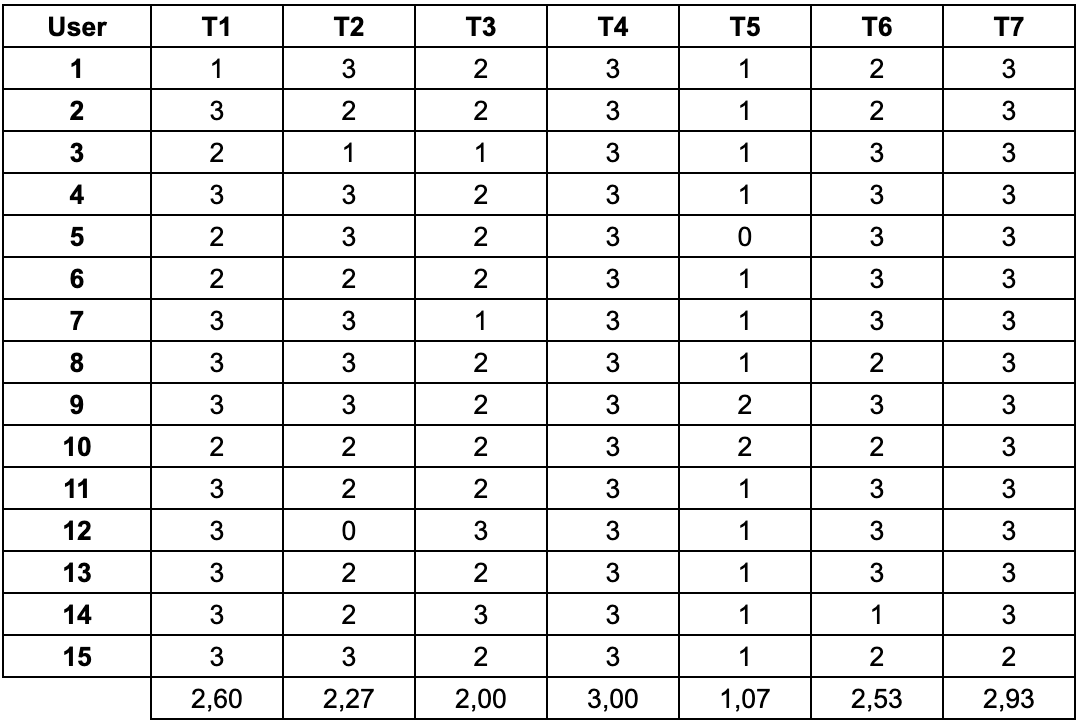
\includegraphics[width=\textwidth]{Images/table1.png}
    \caption{User effectiveness results}
  \end{minipage}
  \hfill
  \begin{minipage}[b]{0.48\textwidth}
    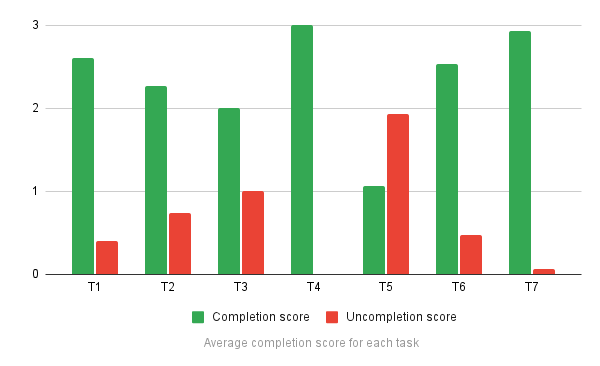
\includegraphics[width=\textwidth]{Images/Eff.png}
    \caption{Average effectiveness per task}
  \end{minipage}
\end{figure}
\\
As shown in the graph we can see that the task with the highest uncompletion score is T5 (airplane ticket information) which required the user to find the FAQs (frequently asked questions) on the website.
This fact clearly highlights the problem that it is not intuitive to find the FAQs page, one that should be immediate to find in order to avoid contacting the assistance.\\
Another task with an alarming uncompletion score is T3 (career fields category). This is a problem related to the design of the Career Fields page and navigation bar menu. When hovering the navigation bar link the website immediately shows all the sub-categories to the user while a more high-granularity filter that allows to select macro-categories is available only inside the page.\\\\
On the other hand, the remaining tasks where managed more easily by the users which means that the application has no relevant problems that prevent these tasks from being completed.

%% --- TOT ---
\paragraph{$\blacksquare$ Efficiency}
System efficiency is measured by the amount of time it takes a user to complete a given tasks. This time is defined as the time that elapses between the opening of the homepage and the instant in which the user completes the activity. The measured times are reported in the following table and they are expressed in seconds.\pagebreak
\begin{figure}[ht]
  \centering
  \begin{minipage}[b]{0.48\textwidth}
    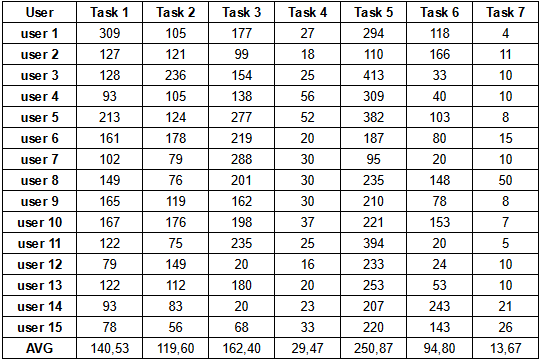
\includegraphics[width=\textwidth]{Images/table2.png}
    \caption{Time on Task in seconds}
  \end{minipage}
  \hfill
  \begin{minipage}[b]{0.48\textwidth}
    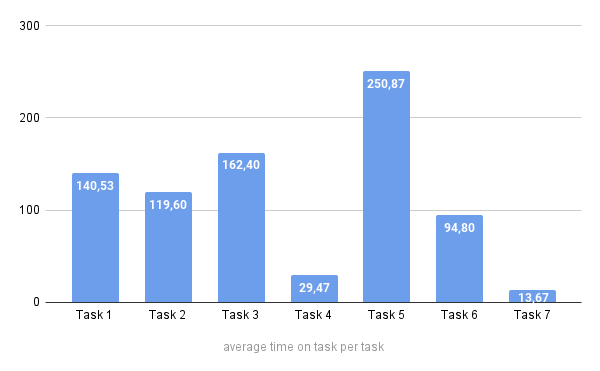
\includegraphics[width=\textwidth]{Images/totAVG.png}
    \caption{Average T.o.T. graph}
  \end{minipage}
\end{figure}\\
The average execution time of the tasks, as shown in the graph 18, appears to be reasonable given the complexity of the tasks. However, from the data, we can observe that T5 (airplane ticket information) is without any doubt the most time-consuming assignment. This is due to the lack of indications in the website on how to find the FAQs which are not immediately visible but and can be found exploring some seemingly unrelated pages.
The experiment also highlights that the users spent most of their time examining the large amount of information that is presented to them, and that is frequently repeated in different pages. This suggests that it might be necessary to reduce the information load on the pages and in the navigation menu.
\\\\
It is also interesting to notice that some users completed T3 (career fields categories) more easily than others, on the other hand we can observe from the individual T.o.T. graph that T5 (airplane ticket information) required each user a significant amount of time.
\begin{figure}[ht]
  \centering
    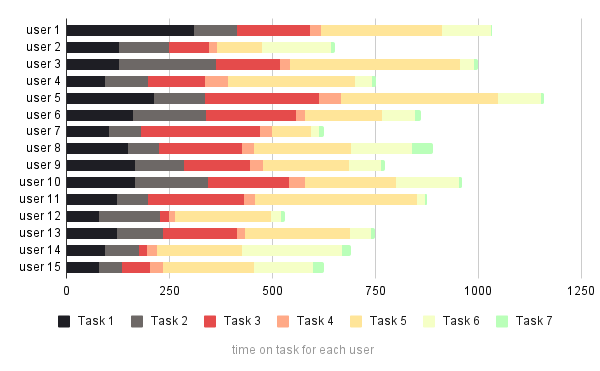
\includegraphics[width=0.8\textwidth]{Images/totUsers.png}
    \caption{Time on Task in seconds per user}
\end{figure}

%% --- User errors and wrong actions ---
\paragraph{$\blacksquare$ Errors and user wrong actions}
The “Number of errors” variable measures the number of wrong actions or paths taken by the user while browsing the website. Here we can observe the values recorded during the execution of the test.
\begin{figure}[ht]
  \centering
  \begin{minipage}[b]{0.48\textwidth}
    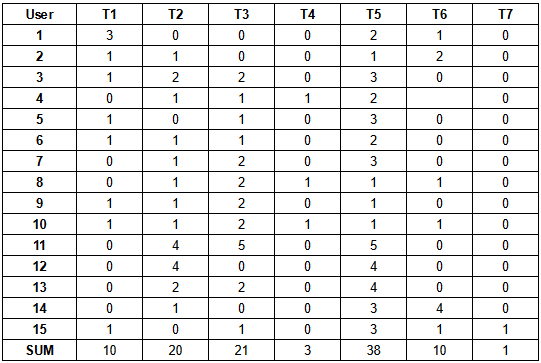
\includegraphics[width=\textwidth]{Images/table3.png}
    \caption{Time on Task in seconds}
  \end{minipage}
  \hfill
  \begin{minipage}[b]{0.48\textwidth}
    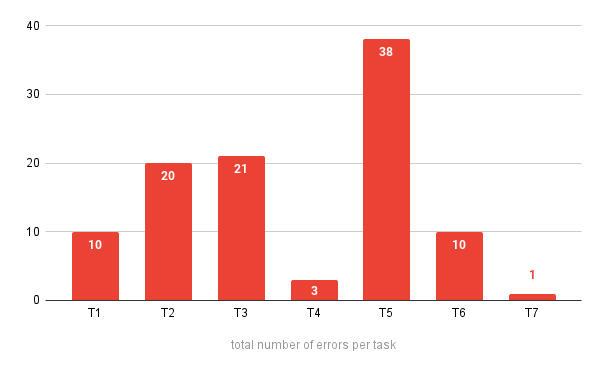
\includegraphics[width=\textwidth]{Images/errors.png}
    \caption{Average T.o.T. graph}
  \end{minipage}
\end{figure}\\
Again, since task T5 (airplane ticket information) is the one with the highest number of errors, it is proven that the FAQs are not easily reachable by the user.
Tasks T3 (career fields categories) and T2 (program fees) are also relevant, since both of them show that the navigation was not found always intuitive by the users.  
As shown in the next sections, some of these issues are confirmed by the answers given in the System Usability Scale questionnaire.

%% --- Perceived task difficulty ---
\paragraph{$\blacksquare$ Perceived task difficulty}
The "Perceived task difficulty" variable allows us to check if the expert observations match with the user feelings towards the website and more specifically towards the tasks they were given.\\
The following graph shows the average perceived difficulty for each task (1 stands for extremely easy and 5 for extremely difficult).
\begin{figure}[ht]
  \centering
    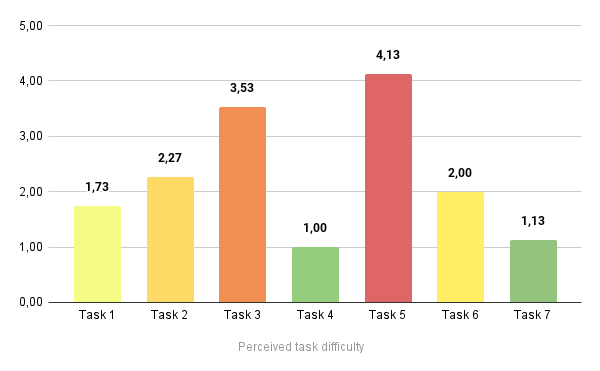
\includegraphics[width=0.6\textwidth]{Images/diff.png}
    \caption{Perceived difficulty for each task}
\end{figure}\\
The results highlight that, as we hypothesized before, the users struggled the most with Tasks T5 (airplane ticket information) and T3 (career fields categories) which are considered difficult.
On the other hand, the remaining tasks were solved more easily by the users, and despite the errors they have committed, mostly on task T2 (program fees), they did not feel like those errors were relevant to their experience with the website and to the task difficulty.
\\Even though, in general, most users quickly understood how the website works, and did not need assistance for the majority of the tasks, they did not enjoy the overall experience and they felt like it would be harder, in particular for less “tech savvy” users to learn how to use the website quickly. This is clearly shown in the following graph, which contains a small section of the System Usability Scale questionnaire.
\begin{figure}[ht]
  \centering
    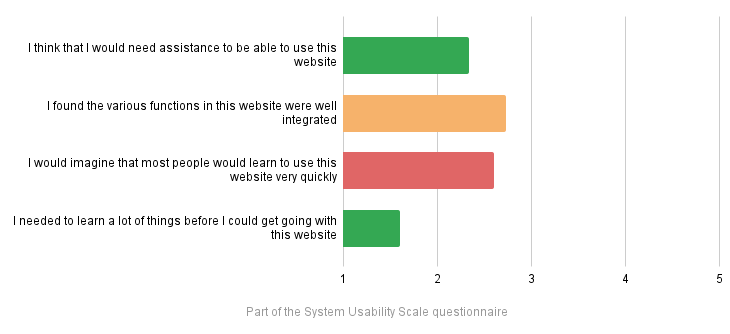
\includegraphics[width=0.9\textwidth]{Images/difficulties.png}
    \caption{User opinions on the website}
\end{figure}

%% --- User satisfaction, disorientation and wandering periods ---
\paragraph{$\blacksquare$ User satisfaction, disorientation and wandering periods}
During the User Testing, the moderators carefully observed the expressions of the users. These data, together with the results of the post-test questionnaires, are essential to assess the degree of satisfaction.
In the graph we can observe the results of most of the System Usability Scale questions, which are fundamental to analyze the user feelings.
\begin{figure}[ht]
  \centering
    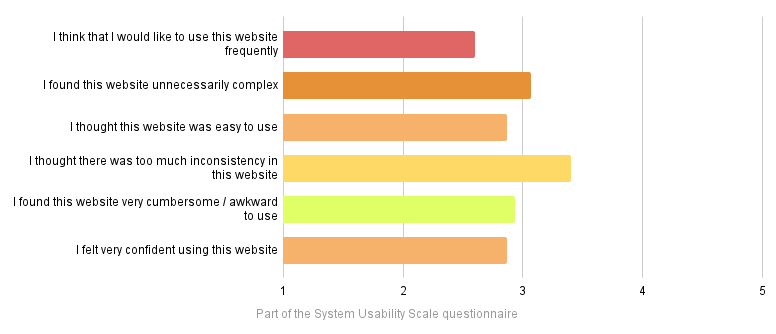
\includegraphics[width=0.9\textwidth]{Images/feelings.png}
    \caption{User opinions on the website}
\end{figure}\\
When solving the easier tasks, most users, did not express disorientation and quickly solved the assignment without noticeable or relevant wandering periods. On the other hand, when the information required were harder to find the users expressed frustration over the lack of clearness in the website menus and the poor implementation of the navigation bar, which was considered “chaotic”.
\\\\
The general opinion on the website is neutral, most users did not complain about the design of the website or the overall appearance. However, they expressed frustration regarding the overwhelming amount of repeated text and the unclear positioning of some key information that is often hidden in secondary pages.
\section{Final Conclusions}
This section discusses the overall conclusions drawn from the study, from both the perspective of the User Testing and Inspection evaluations. Some suggestions for redesign in order to better the usability of the site are also provided.
\subsection{General comments}
After the Inspection and the User Testing, and after having analyzed and discussed together the results, we can now give a general opinion on the website. Both users and experts agreed that product is relatively easy to use and has a nice and a captivating design.
However, it is important to point out that the large amount of frequently repeated information often confuses the user, causing a sense of disorientation and frustration. This vulnerability, among the others we have already discussed before, prevent the website to provide the user an outstanding experience, and should be solved as we will describe in the next section, in order to improve the overall usability of the product.

\subsection{Redesign and Improvements Suggestions}
The following possible improvements have been chosen based on the issues that emerged during the inspection, as well as the suggestions offered by the users that were involved in the testing phase.

\paragraph{Intuitive Navbar Paths Towards Targeted Information}
There are various examples of non-intuitive paths regarding the navbar of the site. This is a great flaw when the main tool users should use to move through the pages is the navbar itself.

\begin{figure}[ht]
  \centering
  \begin{minipage}[b]{0.48\textwidth}
    
\includegraphics[width=0.8\textwidth]{Images/faqs.png}
    \caption{Navbar path towards site FAQs}
  \end{minipage}
  \hfill
  \begin{minipage}[b]{0.48\textwidth}
    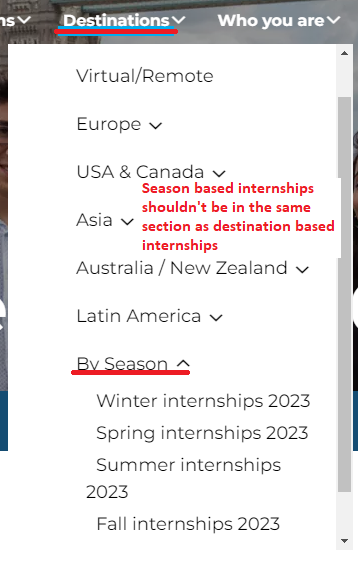
\includegraphics[width=0.8\textwidth]{Images/destinations.png}
    \caption{Navbar path towards season based internships}
  \end{minipage}
\end{figure}

\paragraph{Addition of a Search Bar}
As one of the main functions of the site is to offer information about the services offered by the Intern Group, pages are bound to be content dense. As it's easy for users to feel overwhelmed by the amount of data they are presented, and as the main issues encountered in the Inspection phase regarded content, a \textit{search bar} could be of great aid. Allowing users to directly filter through information through the use of keywords could make users feel in control of the experience, reducing disorientation and dissatisfaction. This suggestion was explicitly given during user testing more than once by the candidates themselves.

\begin{figure}[H]
  \centering
  
\includegraphics[width=\textwidth]{Images/search_bar.png}
  \caption{Search bar placement suggestion}
\end{figure}

\paragraph{Implementing Filtering in Navbar's Career Fields Section}
Another area that was deemed as problematic during all phases of evaluation was the career fields drop-down menu that is accessible from the navbar. Too much information is presented to the user all at once, and there is no clear distinction between career fields that belong to the same category. As a filtering option is already implemented in the Career Fields page, the macro-categories it defines could be shown in said menu so that it produces less information overload. 
\begin{figure}[H]
  \centering
  
\includegraphics[width=\textwidth]{Images/fields.png}
  \caption{Macro-categories offered by the filtering function}
\end{figure}

\newpage

\section{Annex}
\subsection{Heuristics Evaluator Table}
Table of the scores given by each evaluator.
\subsubsection{Presentation Heuristics}
\begin{center}
    \begin{tabular}{|c|c|c|c|c|c|}
        \hline
        \textbf{Code}  & \textbf{Heuristic} & \textbf{Agreed Score} & \textbf{SS} & \textbf{AS} & \textbf{ET} \\
        \hline
        H1 & Visibility of System Status & 2 & 2 & 2 & 3 \\
        \hline
        H2 & Match between the System and the Real World & 5 & 5 & 5 & 5 \\
        \hline
        H5 & Error Prevention & 3 & 4 & 3 & 4 \\
        \hline
        H6 & Recognition rather than Recall & 4 & 5 & 3 & 3 \\
        \hline
        H9 & Help users recognize, diagnose and recover from errors & 2 & 2 & 4 & 2 \\
        \hline
        M7 & Interaction Placeholders - Semiotics & 5 & 5 & 5 & 4 \\
        \hline
        M8 & Interaction Placeholders - Consistency & 4 & 5 & 4 & 5 \\
        \hline
        M9-1 & Spatial Allocation 1 & 5 & 5 & 5 & 4 \\
        \hline
        M9-2 & Spatial Allocation 2 & 5 & 5 & 5 & 4 \\
        \hline
        M10 & Consistency of Page Spatial Structure & 5 & 4 & 5 & 5 \\
        \hline
        M11 & Text Layout & 3 & 2 & 3 & 3 \\
        \hline
        M12 & Consistency of Visual Elements & 4 & 5 & 4 & 4 \\
        \hline
        M13 & Hierarchy 1 & 2 & 2 & 2 & 2 \\
        \hline
        M14 & Hierarchy 2 & 3 & 3 & 3 & 4 \\
        \hline
\end{tabular}
\end{center}

\subsubsection{Navigation Heuristics}
\begin{center}
    \begin{tabular}{|c|c|c|c|c|c|}
        \hline
        \textbf{Code}  & \textbf{Heuristic} & \textbf{Agreed Score} & \textbf{SS} & \textbf{AS} & \textbf{ET} \\
        \hline
        H3 & User Control and Freedom & N/A & N/A & N/A & N/A \\
        \hline
        H7 & Flexibility and Efficiency of Use & 3 & 3 & 3 & 4 \\
        \hline
        M1 & Interaction Consistency & 5 & 5 & 5 & 5 \\
        \hline
        M2-1 & Group Navigation 1 & 4 & 4 & 3 & 4 \\
        \hline
        M2-2 & Group Navigation 2 & 1 & 1 & 1 & 1 \\
        \hline
        M3 & Structural Navigation & 5 & 4 & 4 & 5 \\
        \hline
        M4 & Semantic Navigation & 3 & 3 & 4 & 3 \\
        \hline
        M5 & Landmarks & 4 & 3 & 4 & 3 \\
        \hline
    \end{tabular}
\end{center}

\subsubsection{Content Heuristics}
\begin{center}
    \begin{tabular}{|c|c|c|c|c|c|}
        \hline
        \textbf{Code}  & \textbf{Heuristic} & \textbf{Agreed Score} & \textbf{SS} & \textbf{AS} & \textbf{ET} \\
        \hline
        H8 & Aesthetic and Minimalist Design & 2 & 2 & 1 & 3 \\
        \hline
        H10 & Help and Documentation & N/A & N/A & N/A & N/A \\
        \hline
        M6 & Information Overload & 1 & 1 & 1 & 1 \\
        \hline
        M15 & Consistency of Page Content Structure & 4 & 4 & 3 & 4 \\
        \hline
        M16 & Contextualized Information & 3 & 3 & 3 & 3 \\
        \hline
        M17 & Content Organization (Hierarchy) & 2 & 2 & 2 & 2 \\
        \hline
    \end{tabular}
\end{center}
\subsection{User Testing}
\subsubsection{User Testing by Scherini Samuele}

\begin{figure}[H]
  \centering
  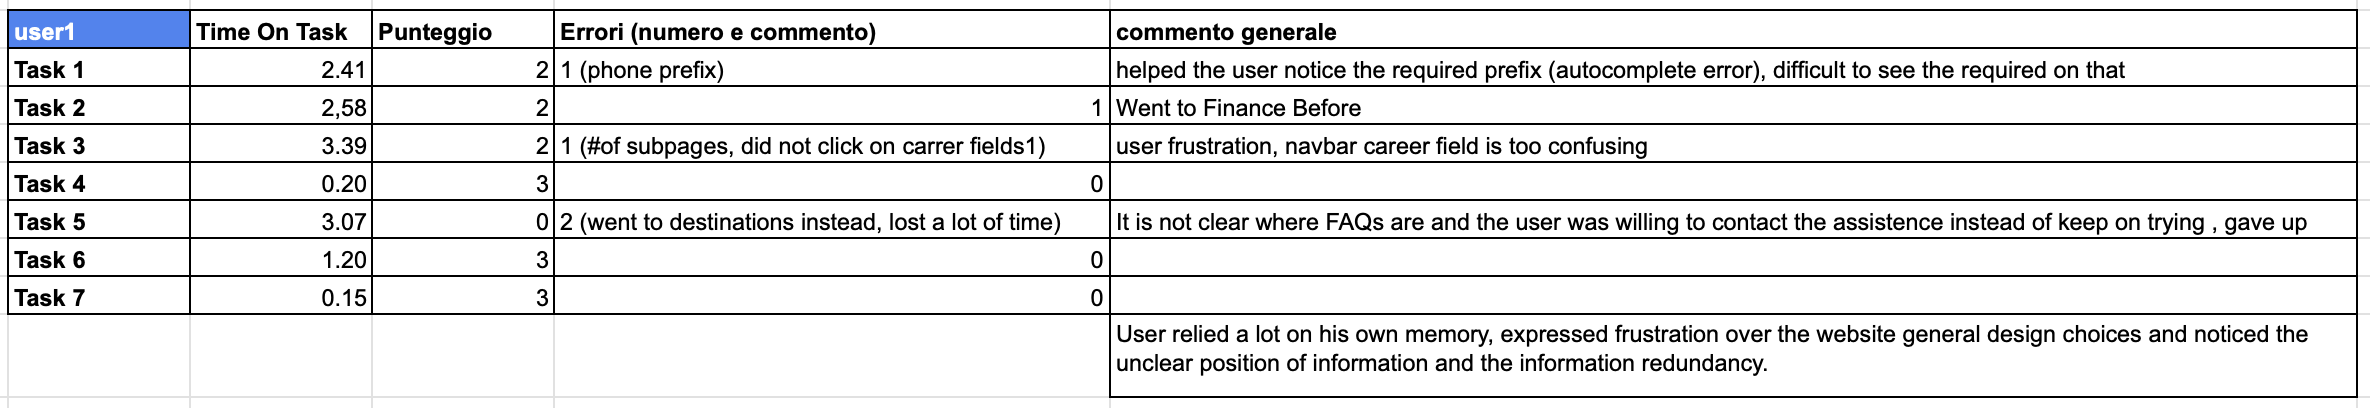
\includegraphics[width=\textwidth]{Images/Test/TestSS1.png}
  \caption{Tester 1 - SS}
\end{figure}

\begin{figure}[H]
  \centering
  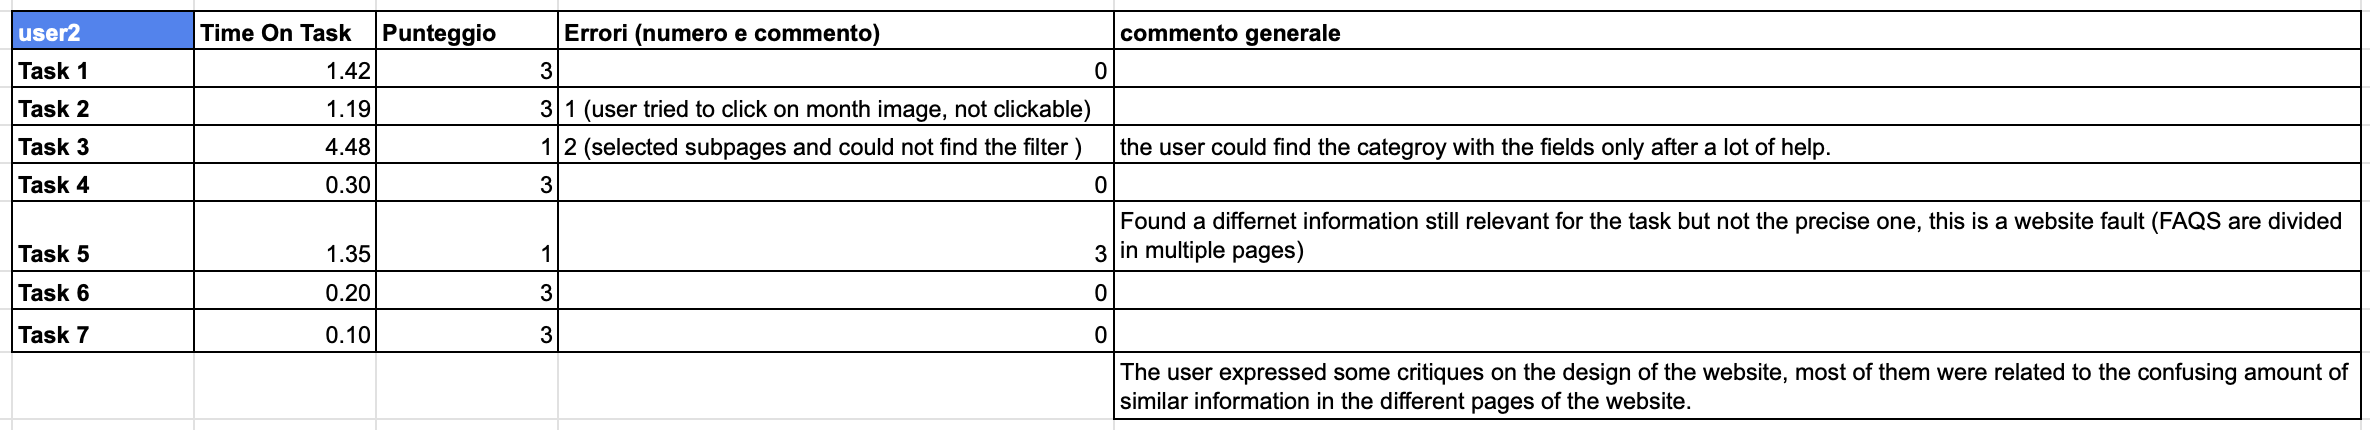
\includegraphics[width=\textwidth]{Images/Test/TestSS2.png}
  \caption{Tester 2 - SS}
\end{figure}

\begin{figure}[H]
  \centering
  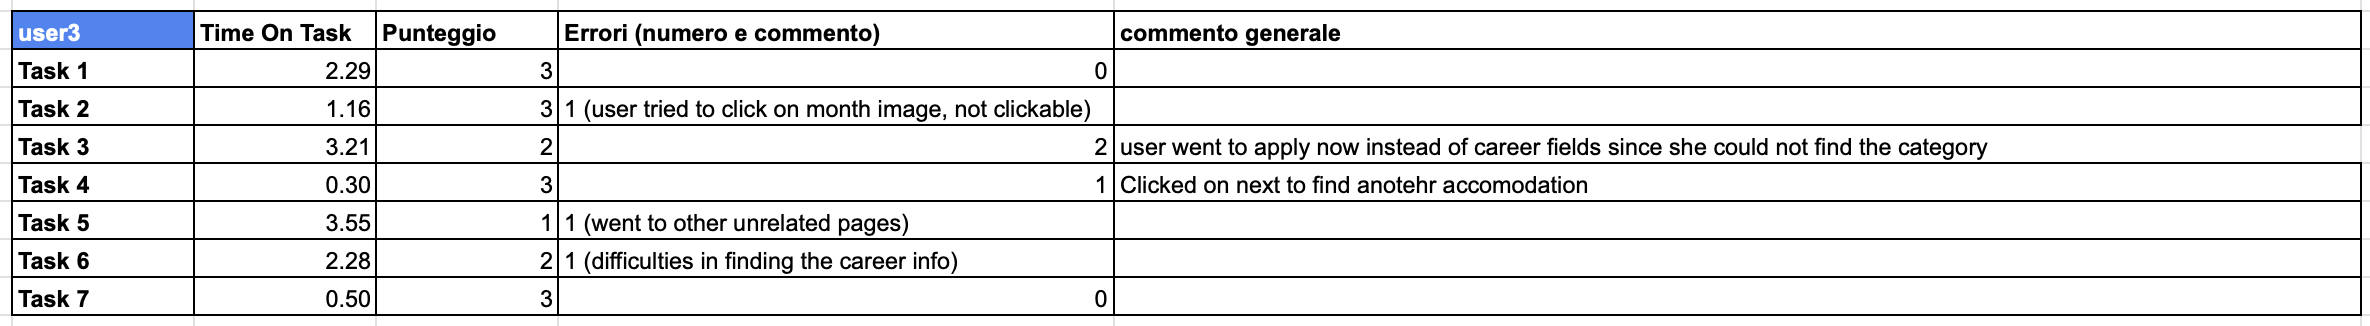
\includegraphics[width=\textwidth]{Images/Test/TestSS3.png}
  \caption{Tester 3 - SS}
\end{figure}

\begin{figure}[H]
  \centering
  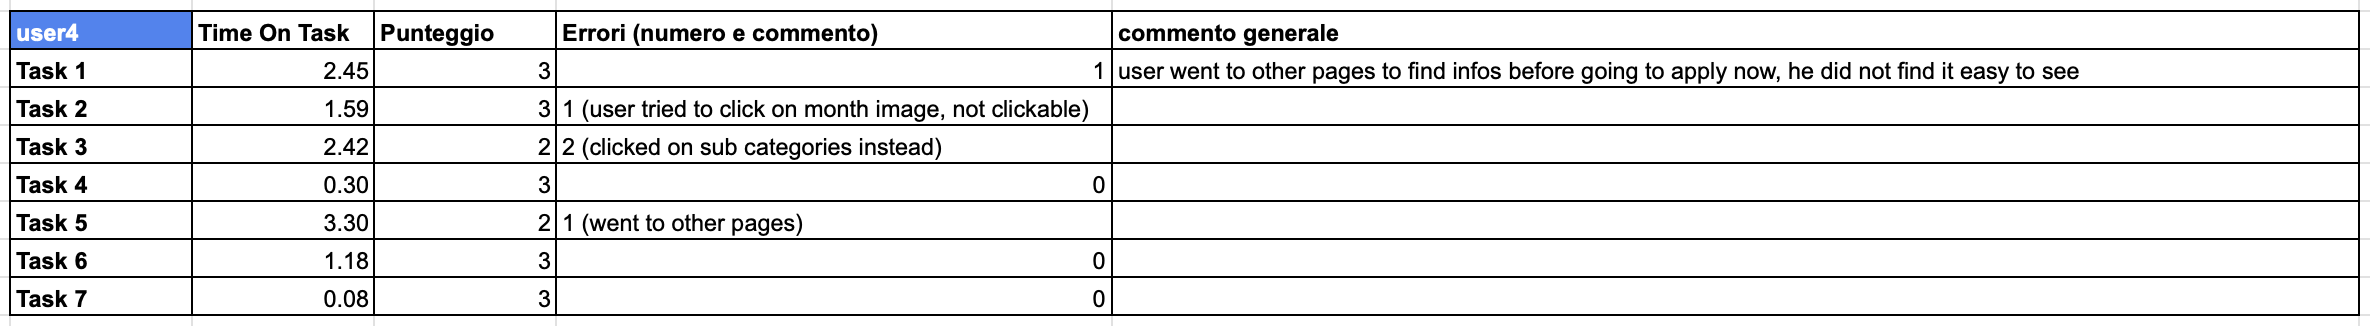
\includegraphics[width=\textwidth]{Images/Test/TestSS4.png}
  \caption{Tester 4 - SS}
\end{figure}

\begin{figure}[H]
  \centering
  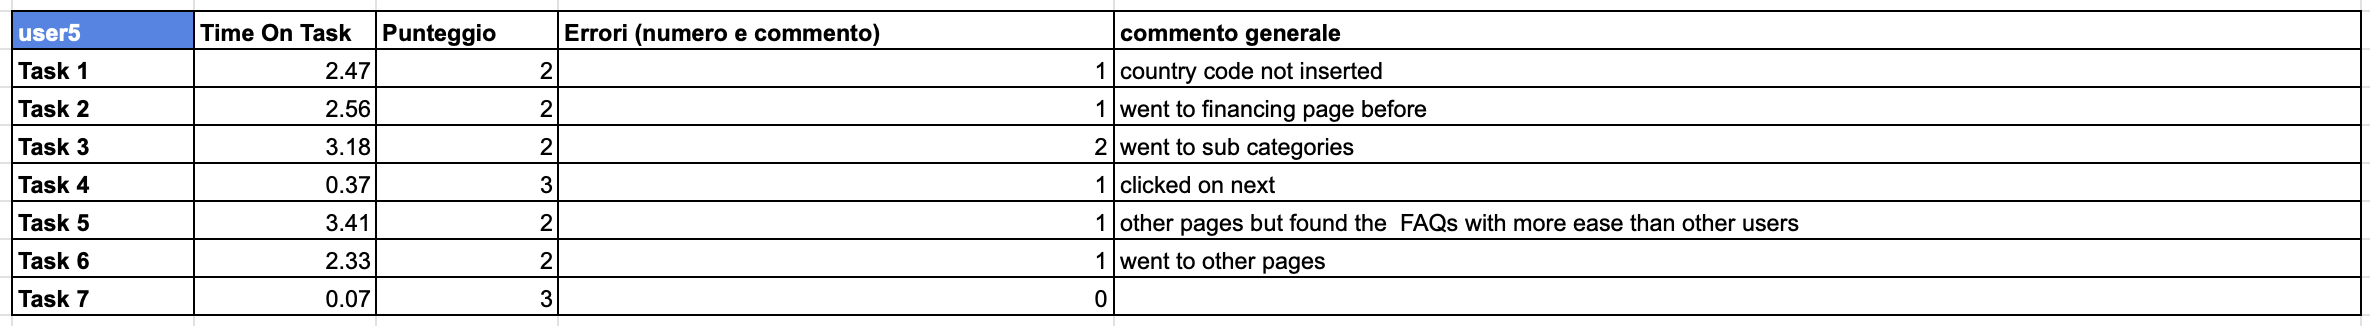
\includegraphics[width=\textwidth]{Images/Test/TestSS5.png}
  \caption{Tester 5 - SS}
\end{figure}

\subsubsection{User Testing by Sironi Alessandro}

\begin{figure}[H]
  \centering
  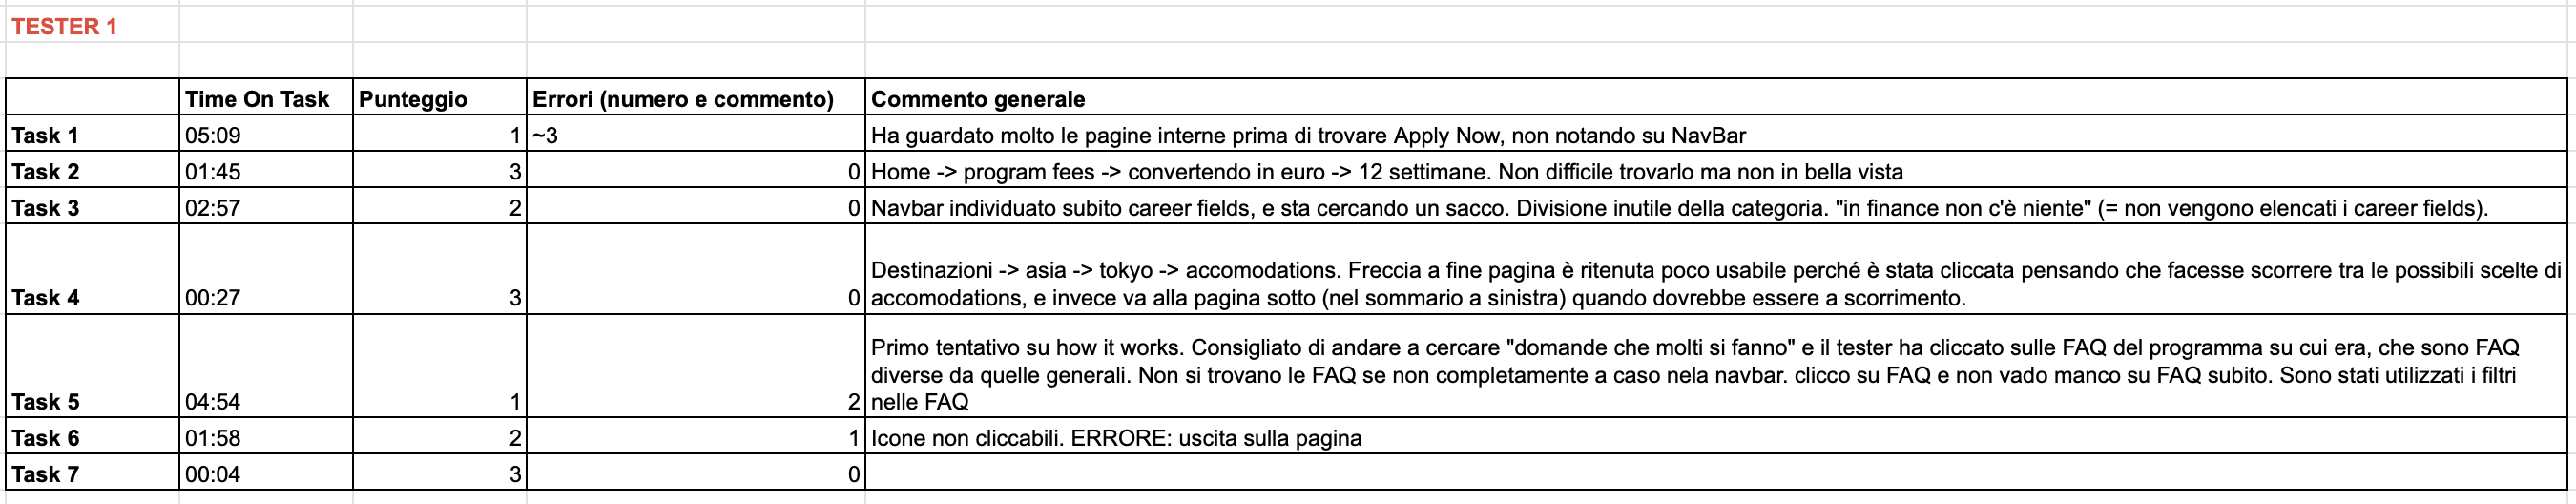
\includegraphics[width=\textwidth]{Images/Test/TestAS1.png}
  \caption{Tester 1 - AS}
\end{figure}

\begin{figure}[H]
  \centering
  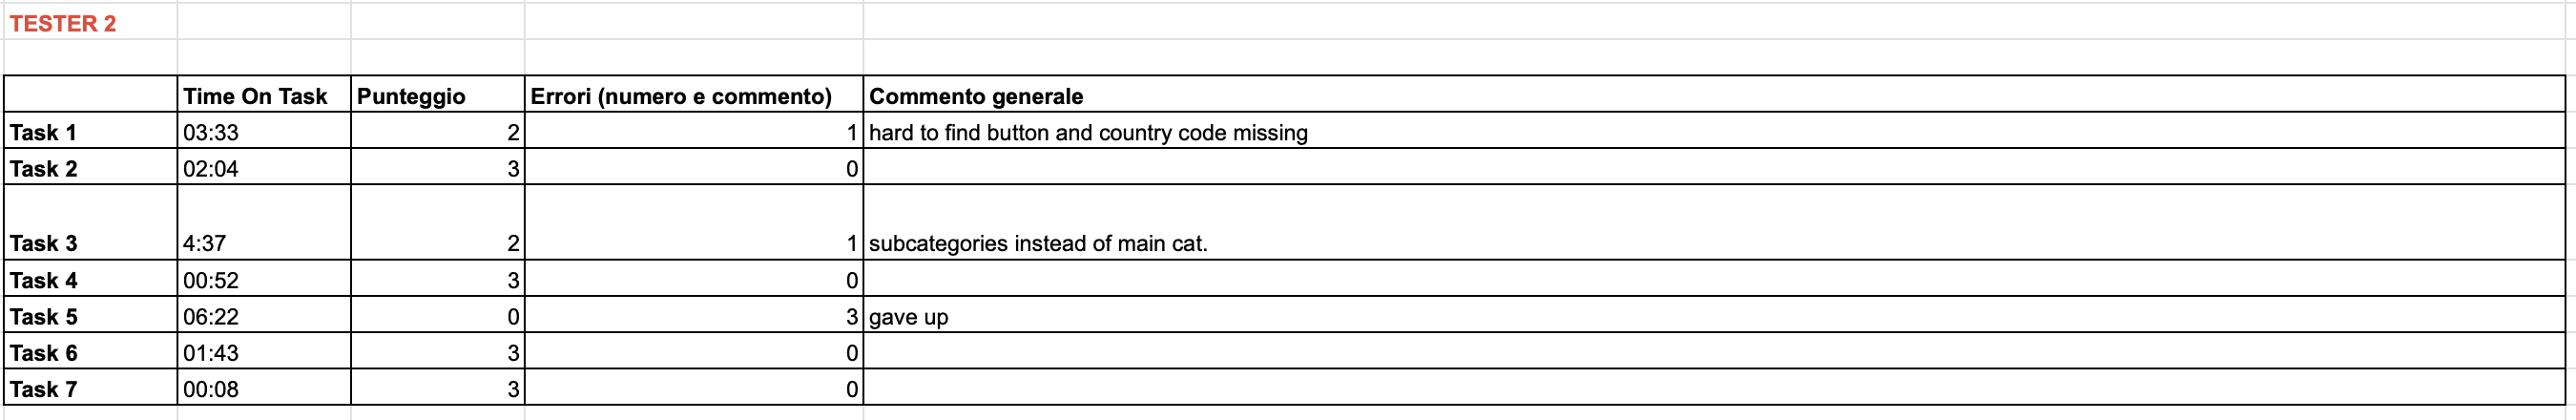
\includegraphics[width=\textwidth]{Images/Test/TestAS2.png}
  \caption{Tester 2 - AS}
\end{figure}

\begin{figure}[H]
  \centering
  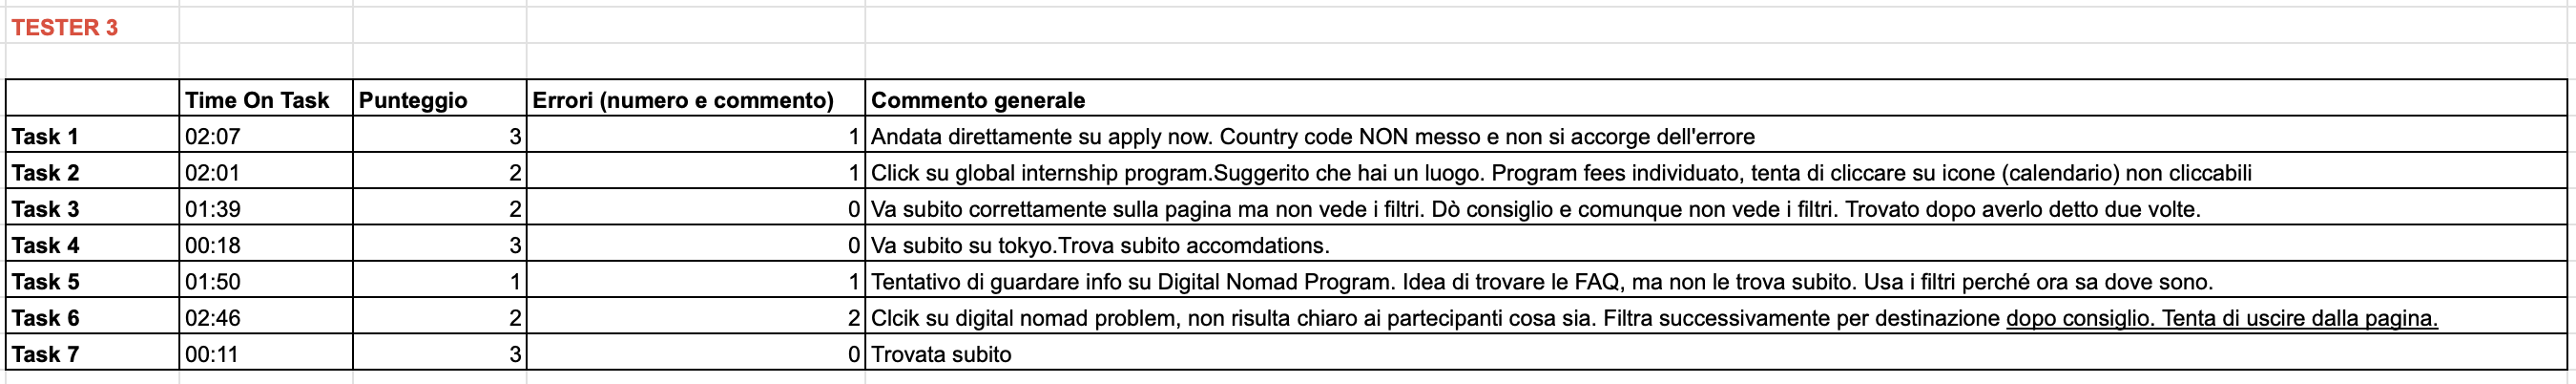
\includegraphics[width=\textwidth]{Images/Test/TestAS3.png}
  \caption{Tester 3 - AS}
\end{figure}

\begin{figure}[H]
  \centering
  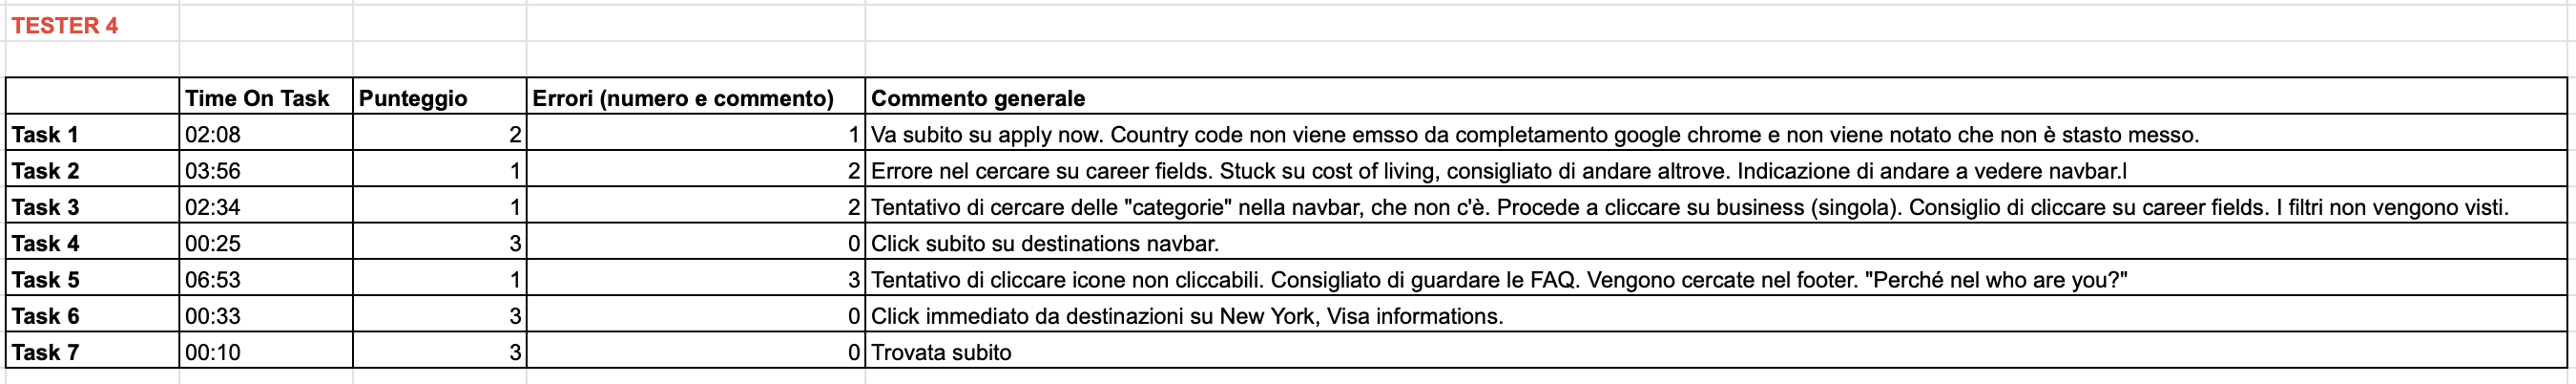
\includegraphics[width=\textwidth]{Images/Test/TestAS4.png}
  \caption{Tester 4 - AS}
\end{figure}

\begin{figure}[H]
  \centering
  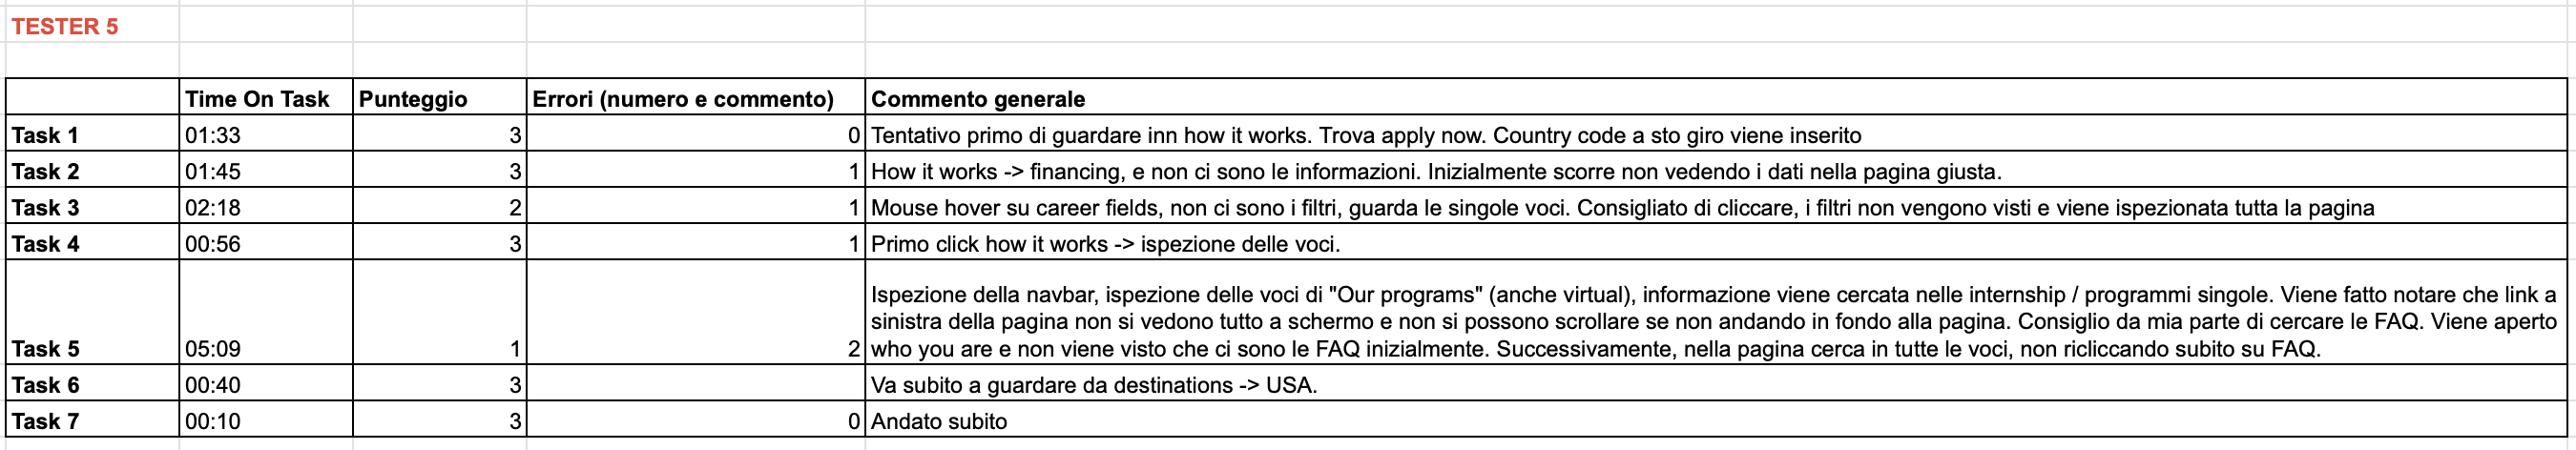
\includegraphics[width=\textwidth]{Images/Test/TestAS5.png}
  \caption{Tester 5 - AS}
\end{figure}

\subsubsection{User Testing by Tognini Elisa}

\begin{figure}[H]
  \centering
  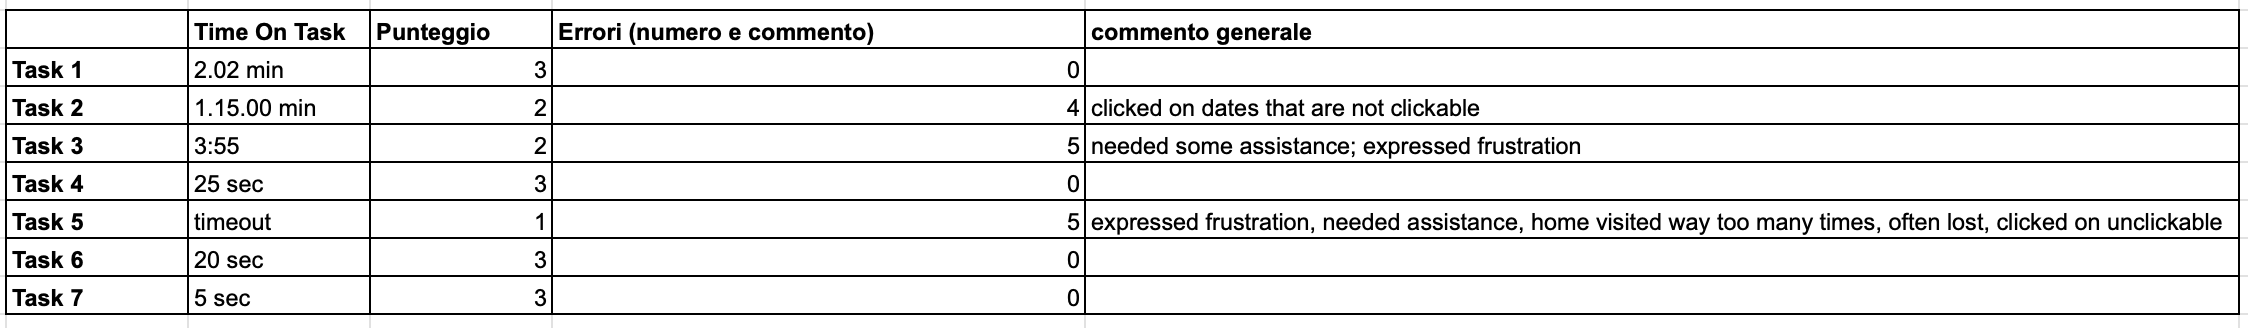
\includegraphics[width=\textwidth]{Images/Test/TestET1.png}
  \caption{Tester 1 - ET}
\end{figure}

\begin{figure}[H]
  \centering
  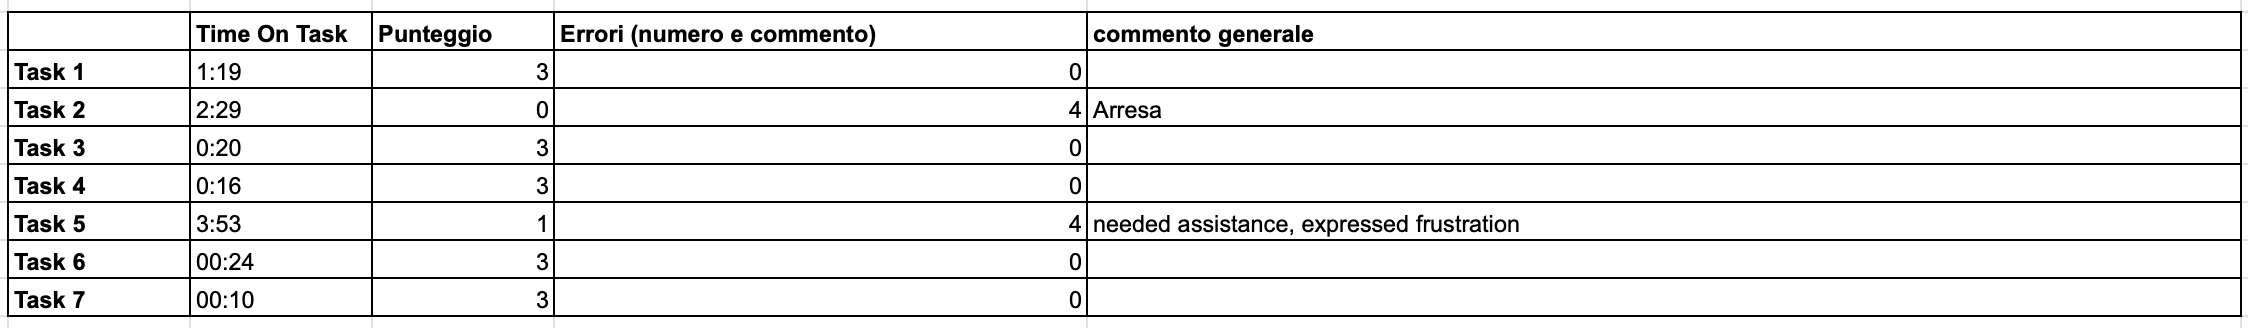
\includegraphics[width=\textwidth]{Images/Test/TestET2.png}
  \caption{Tester 2 - ET}
\end{figure}

\begin{figure}[H]
  \centering
  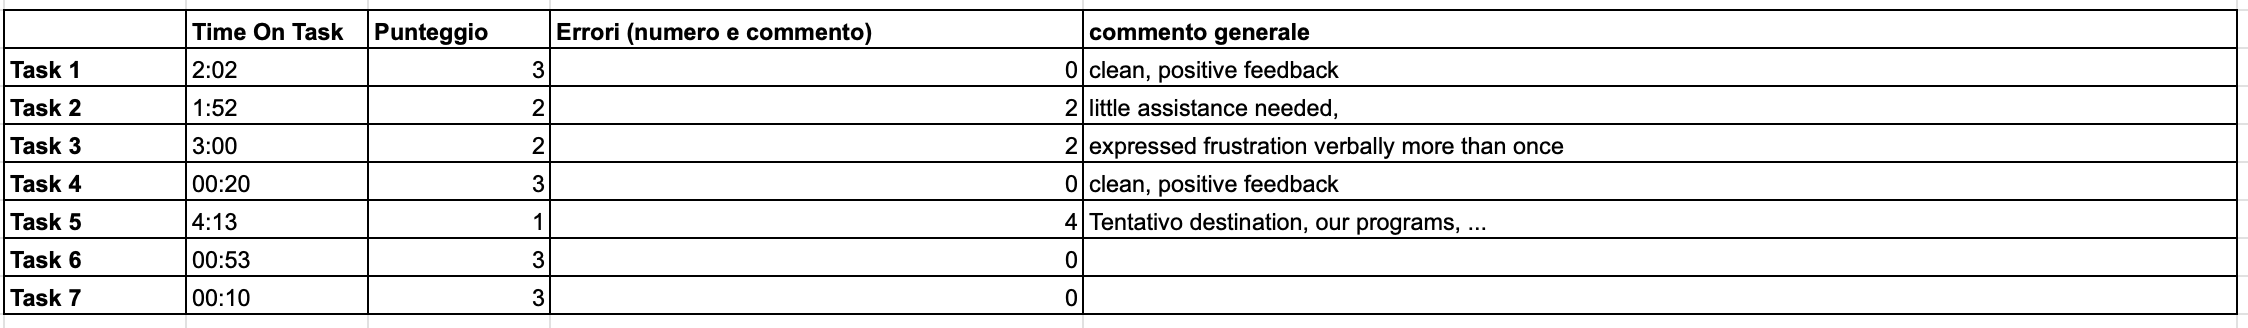
\includegraphics[width=\textwidth]{Images/Test/TestET3.png}
  \caption{Tester 3 - ET}
\end{figure}

\begin{figure}[H]
  \centering
  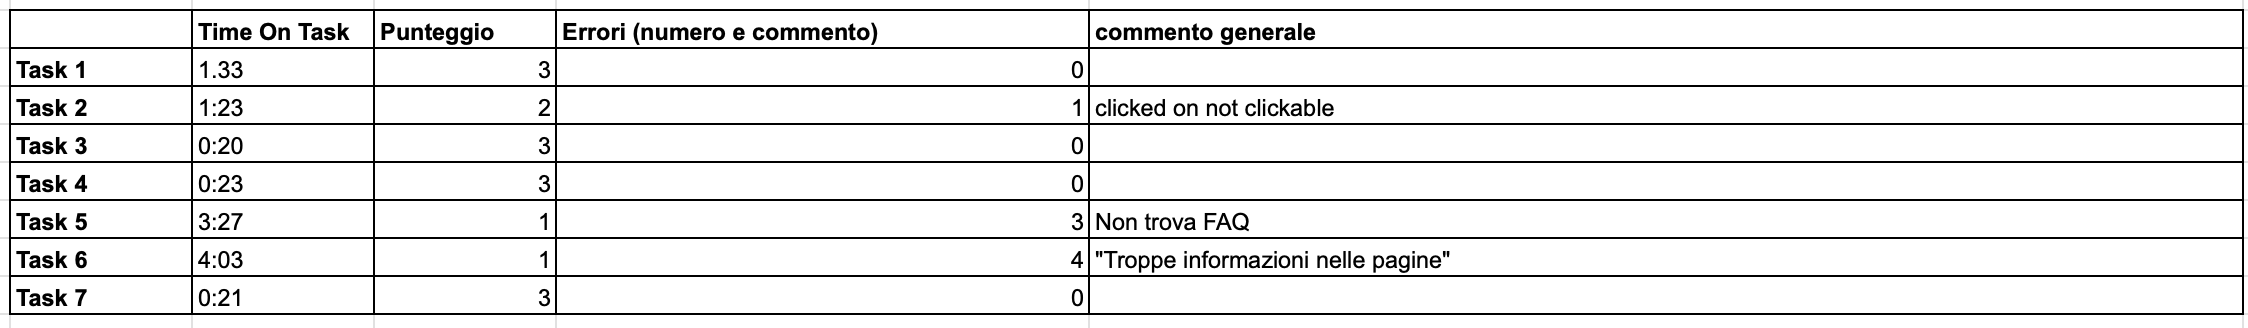
\includegraphics[width=\textwidth]{Images/Test/TestET4.png}
  \caption{Tester 4 - ET}
\end{figure}

\begin{figure}[H]
  \centering
  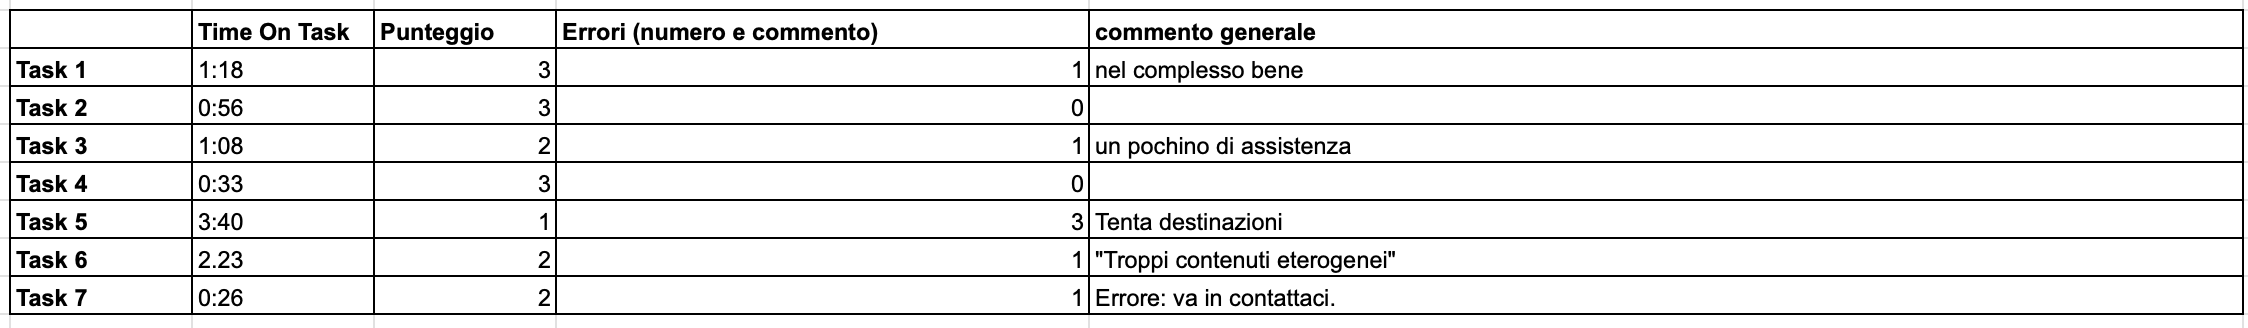
\includegraphics[width=\textwidth]{Images/Test/TestET5.png}
  \caption{Tester 5 - ET}
\end{figure}

\subsection{Division of Labour and Gathering of Data}
The project started with the inspection of the requirements of the project in group. After that, the participants of the group independently scouted the website to find initial hints of problems and to get familiar with the website. 
Together, we then defined the metrics to be used in the evaluations, both from the perspective of the expert and from the tester's.
After that, we designed an internal form to gather the scores of the heuristics and some preliminary comments. We then gathered the data and input it in a spreadsheet.
After this phase, every participant was required to think of a few tasks, that were then finalized as the ones proposed to the testers. 
A few forms designed to be filled by the testers were designed together.
We then administered the tests, each to five testers, independently.
After some aggregation of the data, we started writing this paper. 
For every form that has been used in this project, \textit{Google Forms} was used. \\
Everybody has contributed to every part, but the formal writing was divided in the following way:
\begin{itemize}
    \item User Testing, Conclusions: Scherini Samuele.
    \item Inspection, Conclusions: Sironi Alessandro.
    \item Introduction, Heuristics and Metrics Definition, Conclusions: Tognini Elisa.
\end{itemize}

\end{document}